\documentclass[11pt]{article}
\usepackage[margin=1in]{geometry}
\usepackage{amsmath}
\usepackage{booktabs}
\usepackage{graphicx}
\usepackage{float}
\usepackage{caption}
\usepackage[hidelinks]{hyperref}

\newcommand{\invlogit}{\operatorname{logit}^{-1}}
\newcommand{\code}[1]{\texttt{#1}}

\graphicspath{{Plots_A/Fit_Plots_A/}}

\title{Model A Fit to the Real Data}
\author{Vera Schroeder}
\date{October 2026}

\begin{document}

\maketitle

\section{Summary}

Model A (one psychometric curve per group, with all sessions pooled) was fit to
all 12{,}937 trials of the Sirius data (42 sessions, 4 groups). The main results:

\begin{itemize}
  \item \textbf{The distractor lowers the PSE} by $-4.19$ $\mu m$
        [$-4.96$, $-3.44$] for the left hand and $-6.07$ $\mu m$ [$-6.85$, $-5.30$]
        for the right hand.
  \item \textbf{The distractor raises $\gamma_h$}, the rate of ``high''
        responses to the weakest stimuli, by about 0.04 for both hands.
  \item \textbf{The distractor raises the JND} for the left hand
        (+0.83 $\mu m$ [0.27, 1.37]); for the right hand the HDI includes 0. It
        has no clear effect on $\gamma_l$.
  \item \textbf{The sessions differ more than Model A allows.} Pooled over
        sessions the model reproduces the data at every amplitude, but within
        single sessions, near the threshold, the observed responses vary more than
        Model A predicts. Model A therefore describes these 42 sessions pooled
        together, and its intervals do not include the variation between
        sessions.
\end{itemize}

Every figure and number in this report is produced by
\code{Main\_Analysis\_A.py}; the cell ``Numbers for Fit\_A\_Report.tex'' prints
the numbers that the earlier cells do not. All intervals are 95\% highest
density intervals (HDIs). PSE and JND are in micrometres of stimulus amplitude:
$\text{PSE}_{\mu m} = 28 + 14.63\,\text{PSE}$ and
$\text{JND}_{\mu m} = 14.63\,\text{JND}$, where 28 and 14.63 are the mean and sd
of the 8 amplitude levels.

\section{Model and Fit}

The model is the one described in the Model A convergence report. Each group
$g$ (left\_uni, left\_bi, right\_uni, right\_bi) has one psychometric curve,
\[
  \psi(x) = \gamma_{h,g} + (1 - \gamma_{h,g} - \gamma_{l,g})\,\invlogit(\beta_{0,g} + \beta_{1,g}\,x),
\]
shared by all its trials regardless of session, with the priors
$\beta_0 \sim \mathcal{N}(0, 6)$, $\beta_1 \sim \mathcal{N}(4, 2)$ and
$\gamma_h, \gamma_l = 0.25\,w$ with $w \sim \text{Beta}(\text{mean } 0.2,
\text{ sd } 0.15)$. The lapse prior has mean 0.05, well above the lapse rates found here, but the
data dominate it: the posterior sd of each lapse rate is 5--27\% of its prior
sd, and the PSE and JND posteriors are far narrower than their priors
(Figure~\ref{fig:prior_post_pse}, Appendix~\ref{app:figs}).

The groups have 3{,}230--3{,}237 trials each. The fit used NUTS with 4 chains
of 1000 tuning and 5000 kept draws (20{,}000 draws in total) and took 2.4
minutes.

\subsection{Sampling diagnostics}

There were no divergences, and the tree depth never exceeded 5. All 40
parameters have $\hat{R} = 1.000$, bulk ESS $\ge 15{,}213$ and tail ESS
$\ge 8{,}802$. The chains overlap completely (Figure~\ref{fig:trace}).

\begin{figure}[H]
\centering
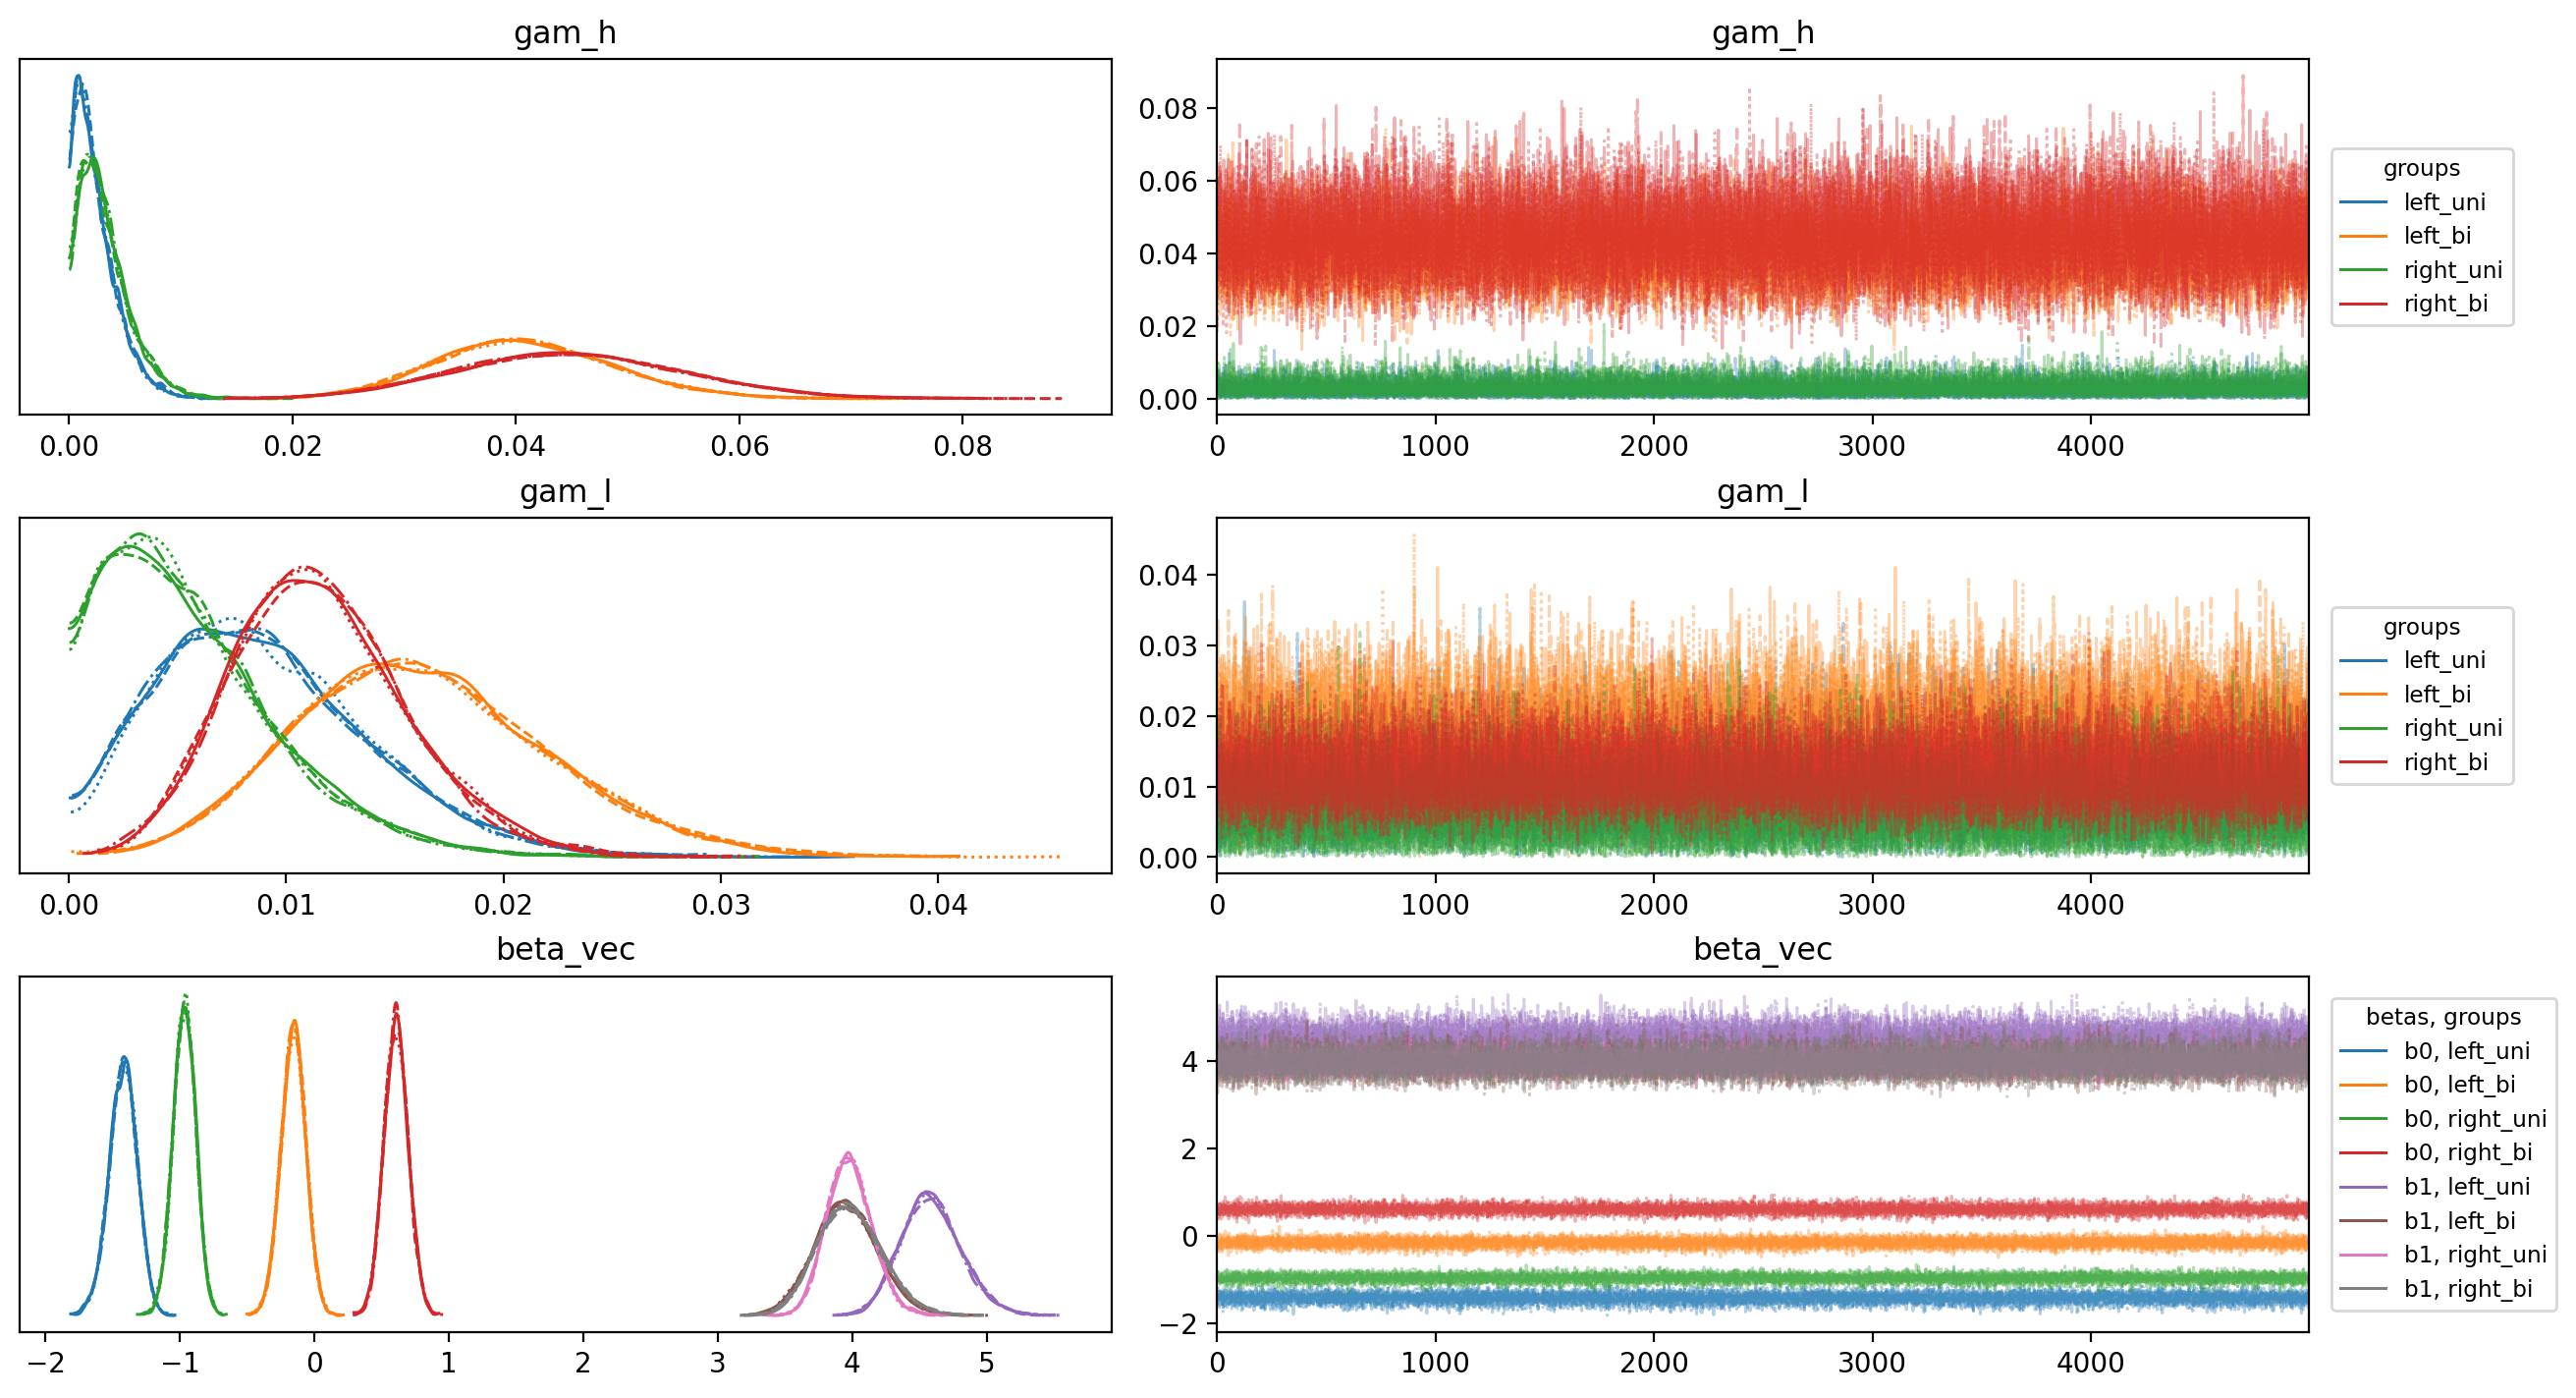
\includegraphics[width=\textwidth]{trace_all_groups.png}
\caption{Trace plots of $\gamma_h$, $\gamma_l$, $\beta_0$ and $\beta_1$ for all
groups (left: density per chain; right: draws).}
\label{fig:trace}
\end{figure}

\section{Group Estimates}

\begin{table}[H]
\centering
\caption{Posterior mean [95\% HDI] of the psychometric quantities of each
group.}
\label{tab:groups}
\resizebox{\textwidth}{!}{%
\begin{tabular}{lcccc}
\toprule
 & PSE ($\mu m$) & JND ($\mu m$) & $\gamma_h$ & $\gamma_l$ \\
\midrule
left\_uni  & 32.58 [32.10, 33.04] & 3.56 [3.25, 3.89] & 0.002 [0.000, 0.006] & 0.009 [0.000, 0.018] \\
left\_bi   & 28.38 [27.79, 28.98] & 4.39 [3.93, 4.83] & 0.041 [0.025, 0.056] & 0.016 [0.005, 0.027] \\
right\_uni & 31.57 [31.05, 32.06] & 4.09 [3.77, 4.41] & 0.003 [0.000, 0.008] & 0.006 [0.000, 0.013] \\
right\_bi  & 25.50 [24.89, 26.08] & 4.36 [3.93, 4.81] & 0.045 [0.025, 0.064] & 0.012 [0.004, 0.020] \\
\bottomrule
\end{tabular}}
\end{table}

\begin{figure}[H]
\centering
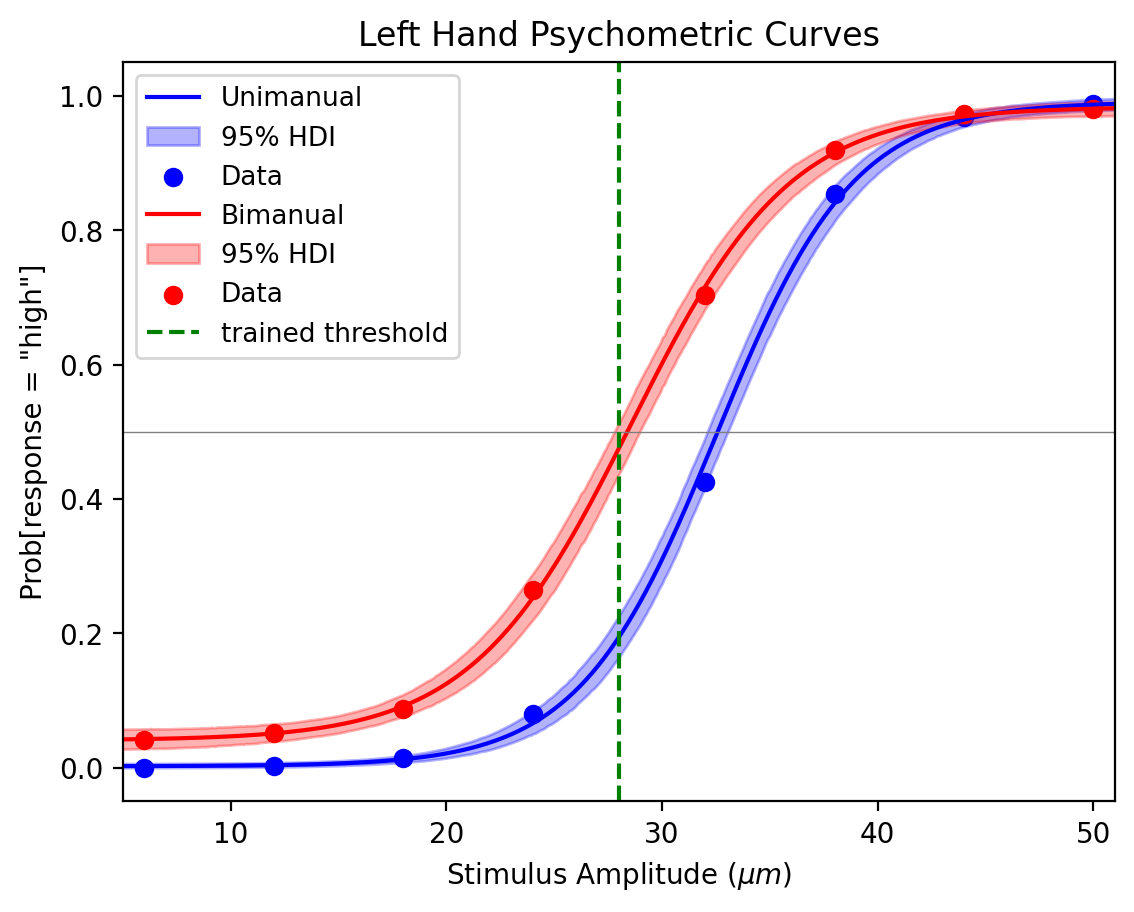
\includegraphics[width=0.48\textwidth]{curves_left.png}\hfill
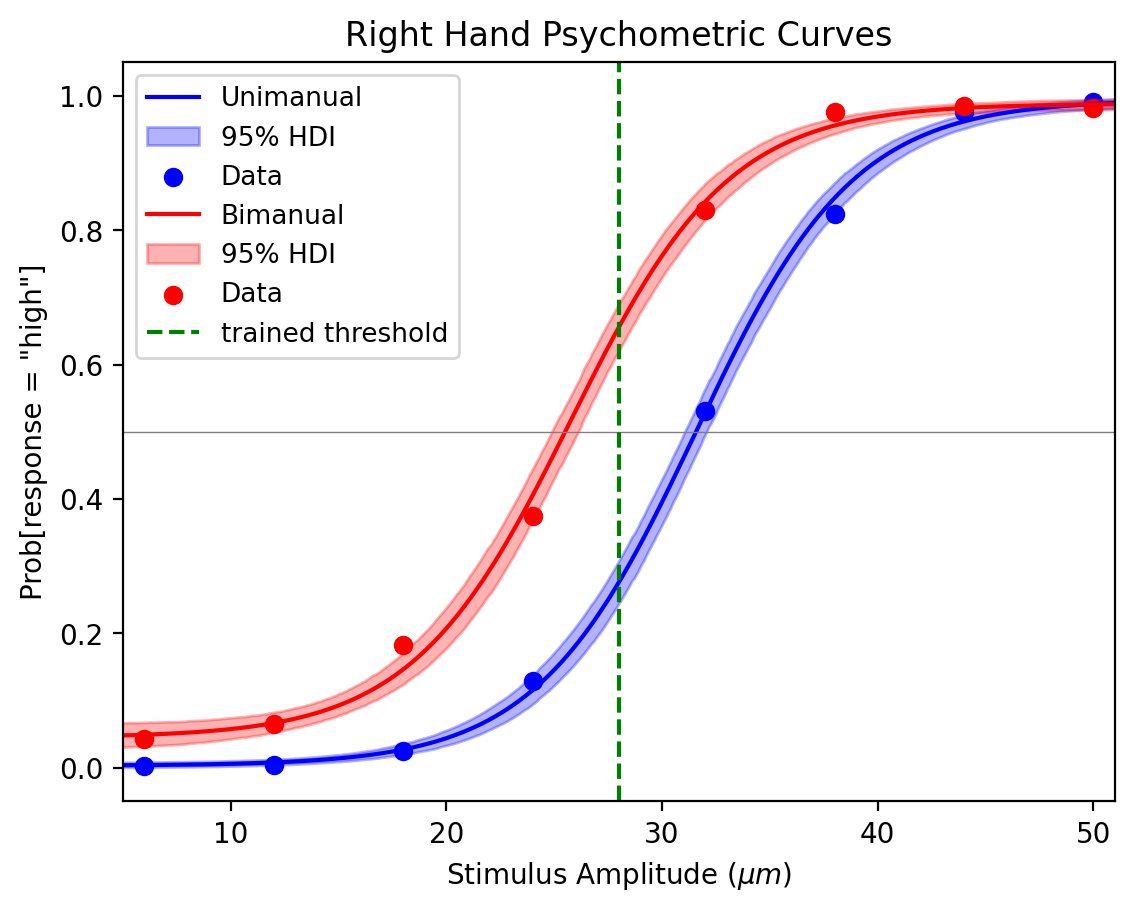
\includegraphics[width=0.48\textwidth]{curves_right.png}
\caption{Fitted psychometric curves (at the posterior means of the parameters,
with the pointwise 95\% HDI of the curve) and the observed proportions of
``high'' responses, pooled over sessions. Unimanual in blue, bimanual in red;
the dashed line is the trained threshold of 28 $\mu m$.}
\label{fig:curves}
\end{figure}

Without the distractor the PSE lies 4.6 (left) and 3.6 (right) $\mu m$ above the
trained threshold: the monkey needs a slightly stronger stimulus than the
trained boundary before it reports ``high''. With the distractor the PSE moves
to the threshold (left hand) or below it (right hand). Lapse rates are small;
$\gamma_h$ is close to 0 without the distractor and about 0.04 with it.

The Model A convergence study found that, at this data size and when the model
is correct, the PSE, JND and $\gamma_h$ are recovered without bias and with
calibrated HDIs, while small values of $\gamma_l$ are pulled upward by the
prior. The $\gamma_l$ estimates of 0.006--0.016 are therefore upper-leaning.

\begin{figure}[H]
\centering
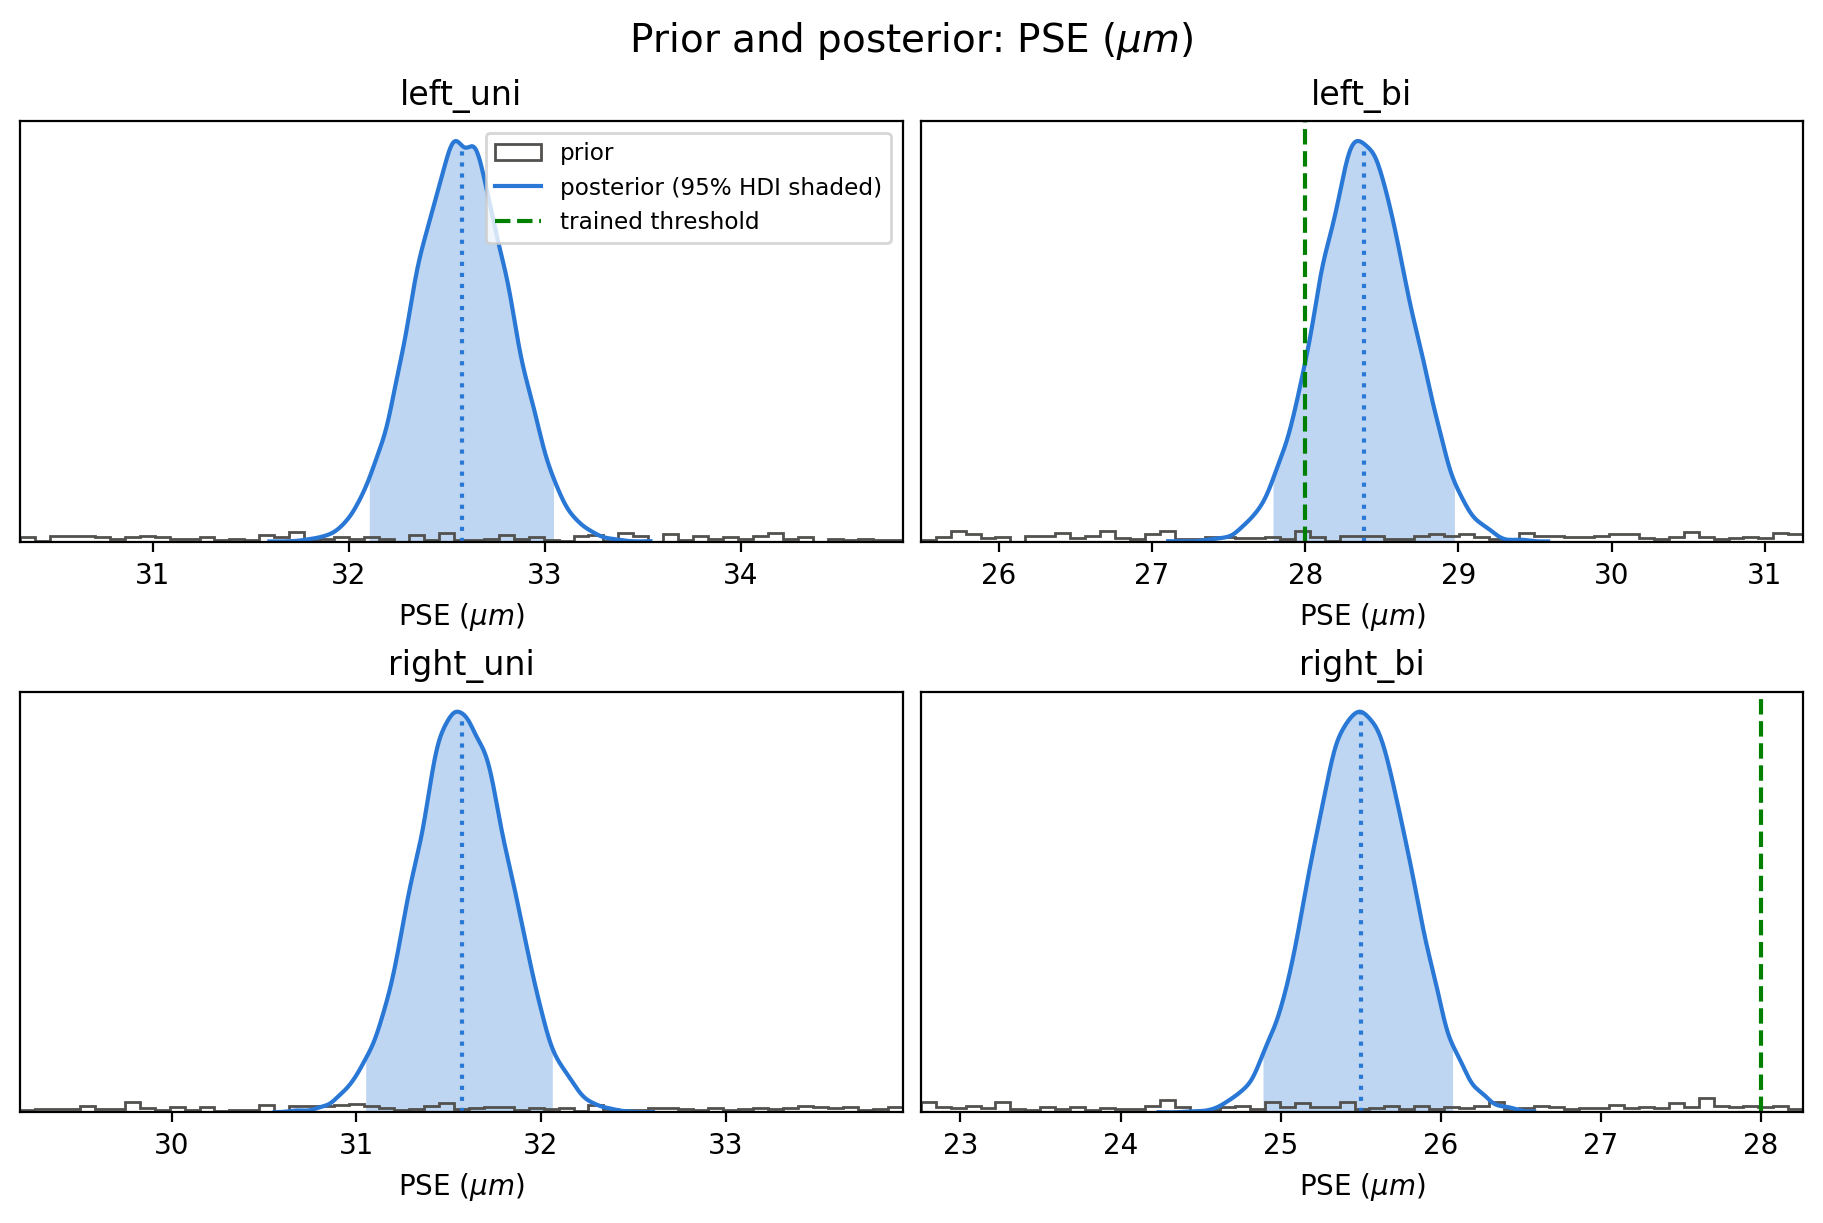
\includegraphics[width=0.8\textwidth]{prior_post_PSE.png}
\caption{Prior (gray) and posterior (blue) of the PSE in each group.}
\label{fig:prior_post_pse}
\end{figure}

\section{Effect of the Distractor}

The effect of the distractor is the bimanual $-$ unimanual difference, computed
draw by draw so that its uncertainty is exact.

\begin{table}[H]
\centering
\caption{Distractor effect (bimanual $-$ unimanual) under Model A: posterior mean
[95\% HDI] and the posterior probability that the effect is positive.}
\label{tab:effect}
\begin{tabular}{llcc}
\toprule
Hand & Quantity & effect & $P(\text{effect} > 0)$ \\
\midrule
Left  & PSE ($\mu m$) & $-4.19$ [$-4.96$, $-3.44$] & 0.000 \\
      & JND ($\mu m$) & 0.83 [0.27, 1.37] & 0.998 \\
      & $\gamma_h$    & 0.038 [0.023, 0.055] & 1.000 \\
      & $\gamma_l$    & 0.007 [$-0.008$, 0.022] & 0.832 \\
\midrule
Right & PSE ($\mu m$) & $-6.07$ [$-6.85$, $-5.30$] & 0.000 \\
      & JND ($\mu m$) & 0.27 [$-0.29$, 0.80] & 0.837 \\
      & $\gamma_h$    & 0.042 [0.021, 0.061] & 1.000 \\
      & $\gamma_l$    & 0.006 [$-0.006$, 0.017] & 0.858 \\
\bottomrule
\end{tabular}
\end{table}

\begin{figure}[H]
\centering
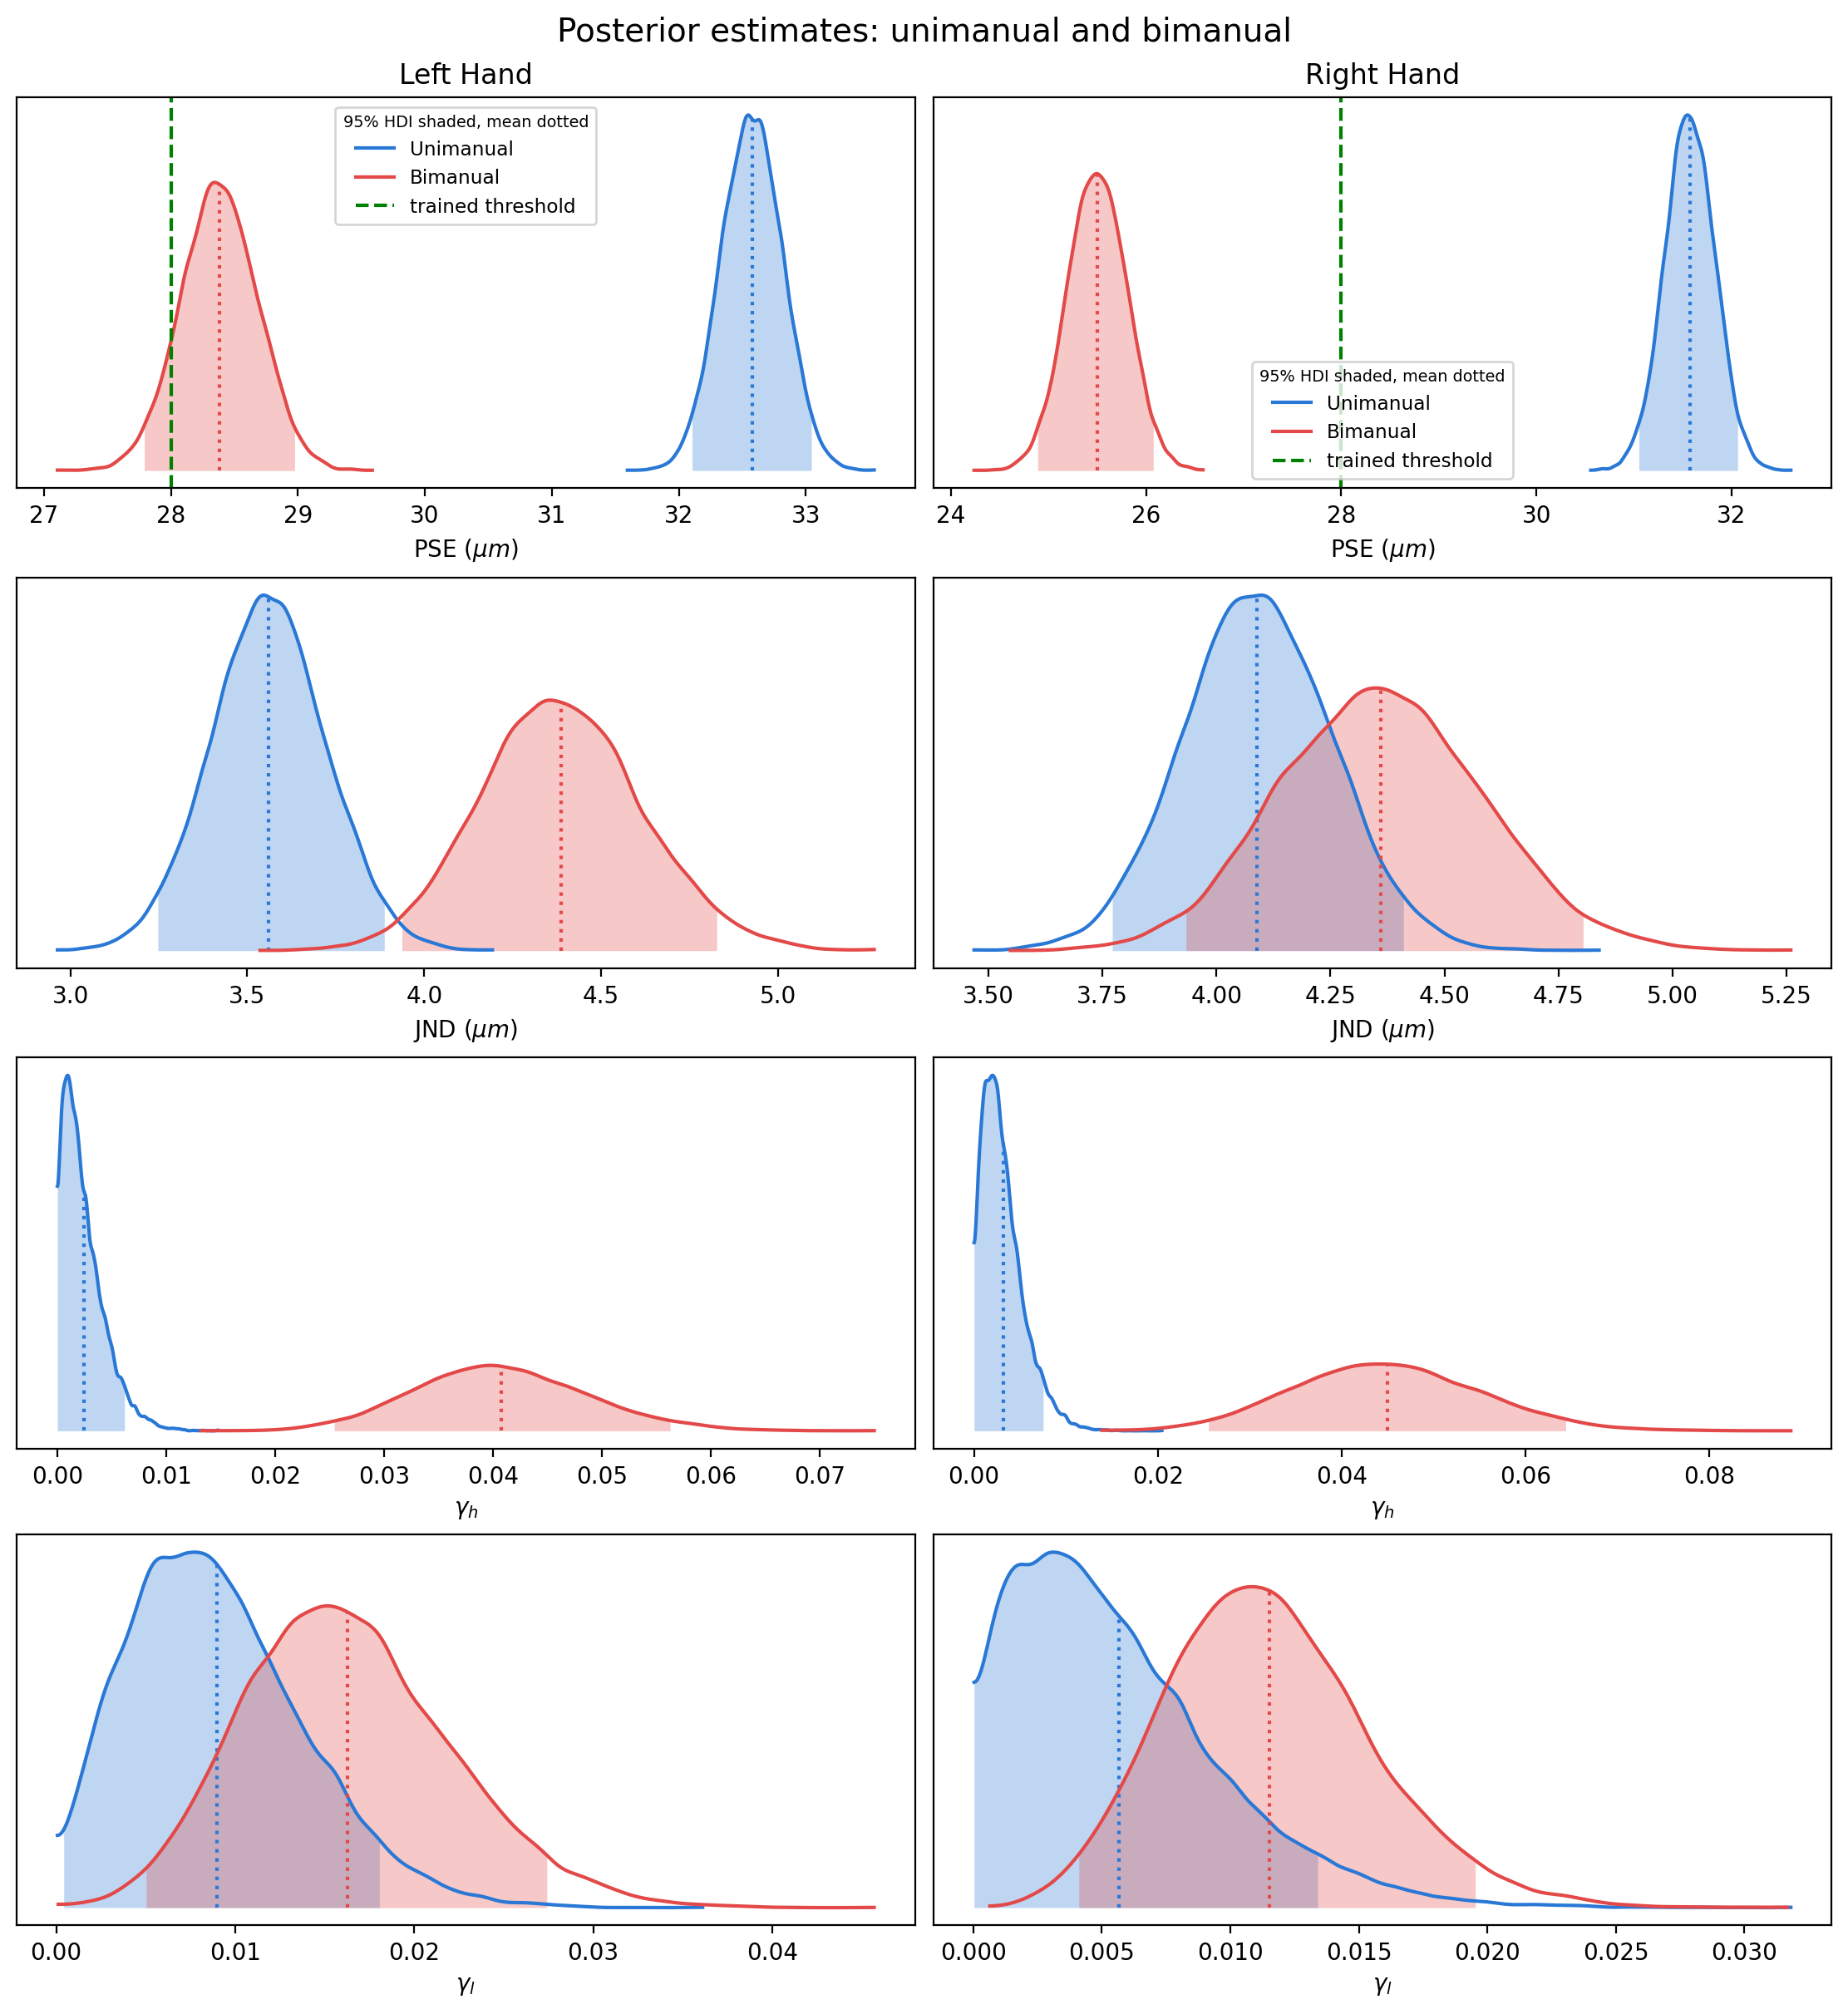
\includegraphics[width=0.9\textwidth]{uni_bi_posteriors.png}
\caption{Posteriors of PSE, JND, $\gamma_h$ and $\gamma_l$ for the unimanual
(blue) and bimanual (red) condition of each hand, with 95\% HDIs shaded.}
\label{fig:uni_bi}
\end{figure}

\begin{figure}[H]
\centering
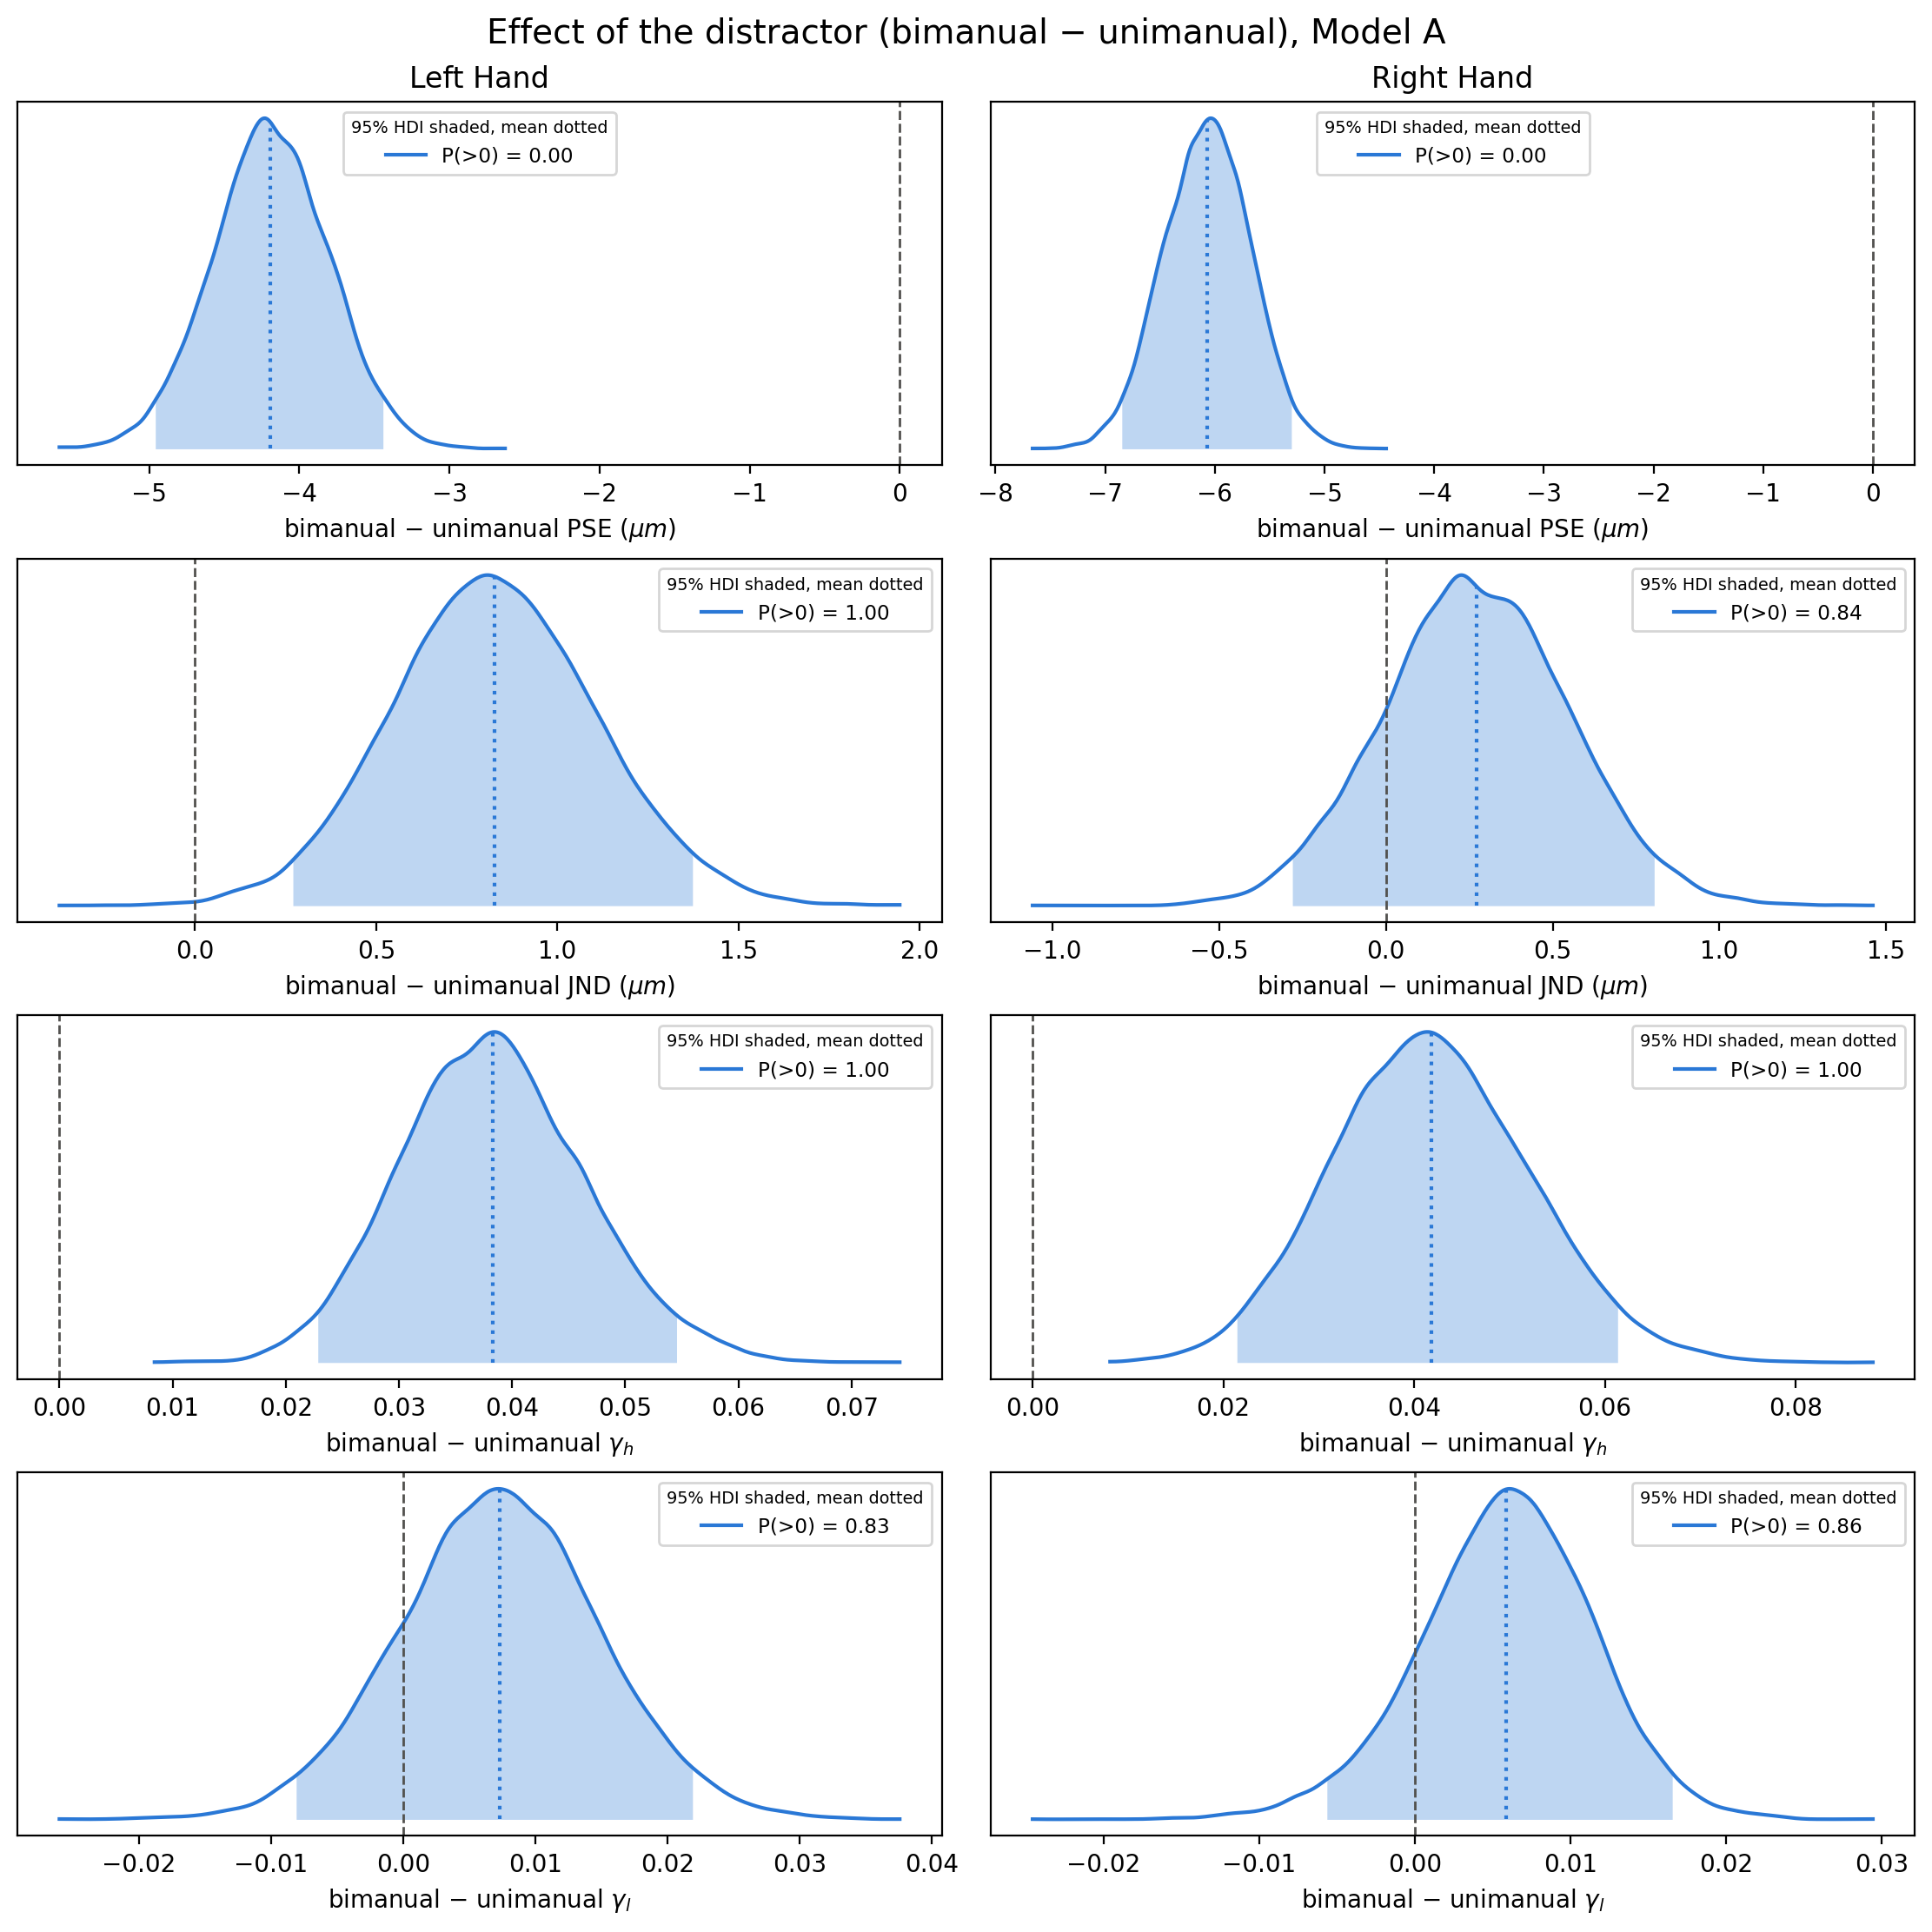
\includegraphics[width=0.9\textwidth]{effect_densities.png}
\caption{Posterior of the distractor effect (bimanual $-$ unimanual), with the
95\% HDI shaded and the posterior probability that the effect is positive.}
\label{fig:effect}
\end{figure}

The distractor shifts the PSE down by 4--6 $\mu m$ and raises $\gamma_h$ by
about 0.04, both with probability essentially 1 (Table~\ref{tab:effect},
Figures~\ref{fig:uni_bi} and~\ref{fig:effect}): with a distractor on the other
hand the monkey reports ``high'' at lower amplitudes, and occasionally even for
the weakest stimuli. The JND rises by 0.83 $\mu m$ for the left hand
($P > 0$: 0.998); for the right hand the rise of 0.27 $\mu m$ is uncertain
($P > 0$: 0.84). Any effect on $\gamma_l$ is small and uncertain.

\section{Model Checks}

\subsection{Posterior predictive checks}

\begin{figure}[H]
\centering
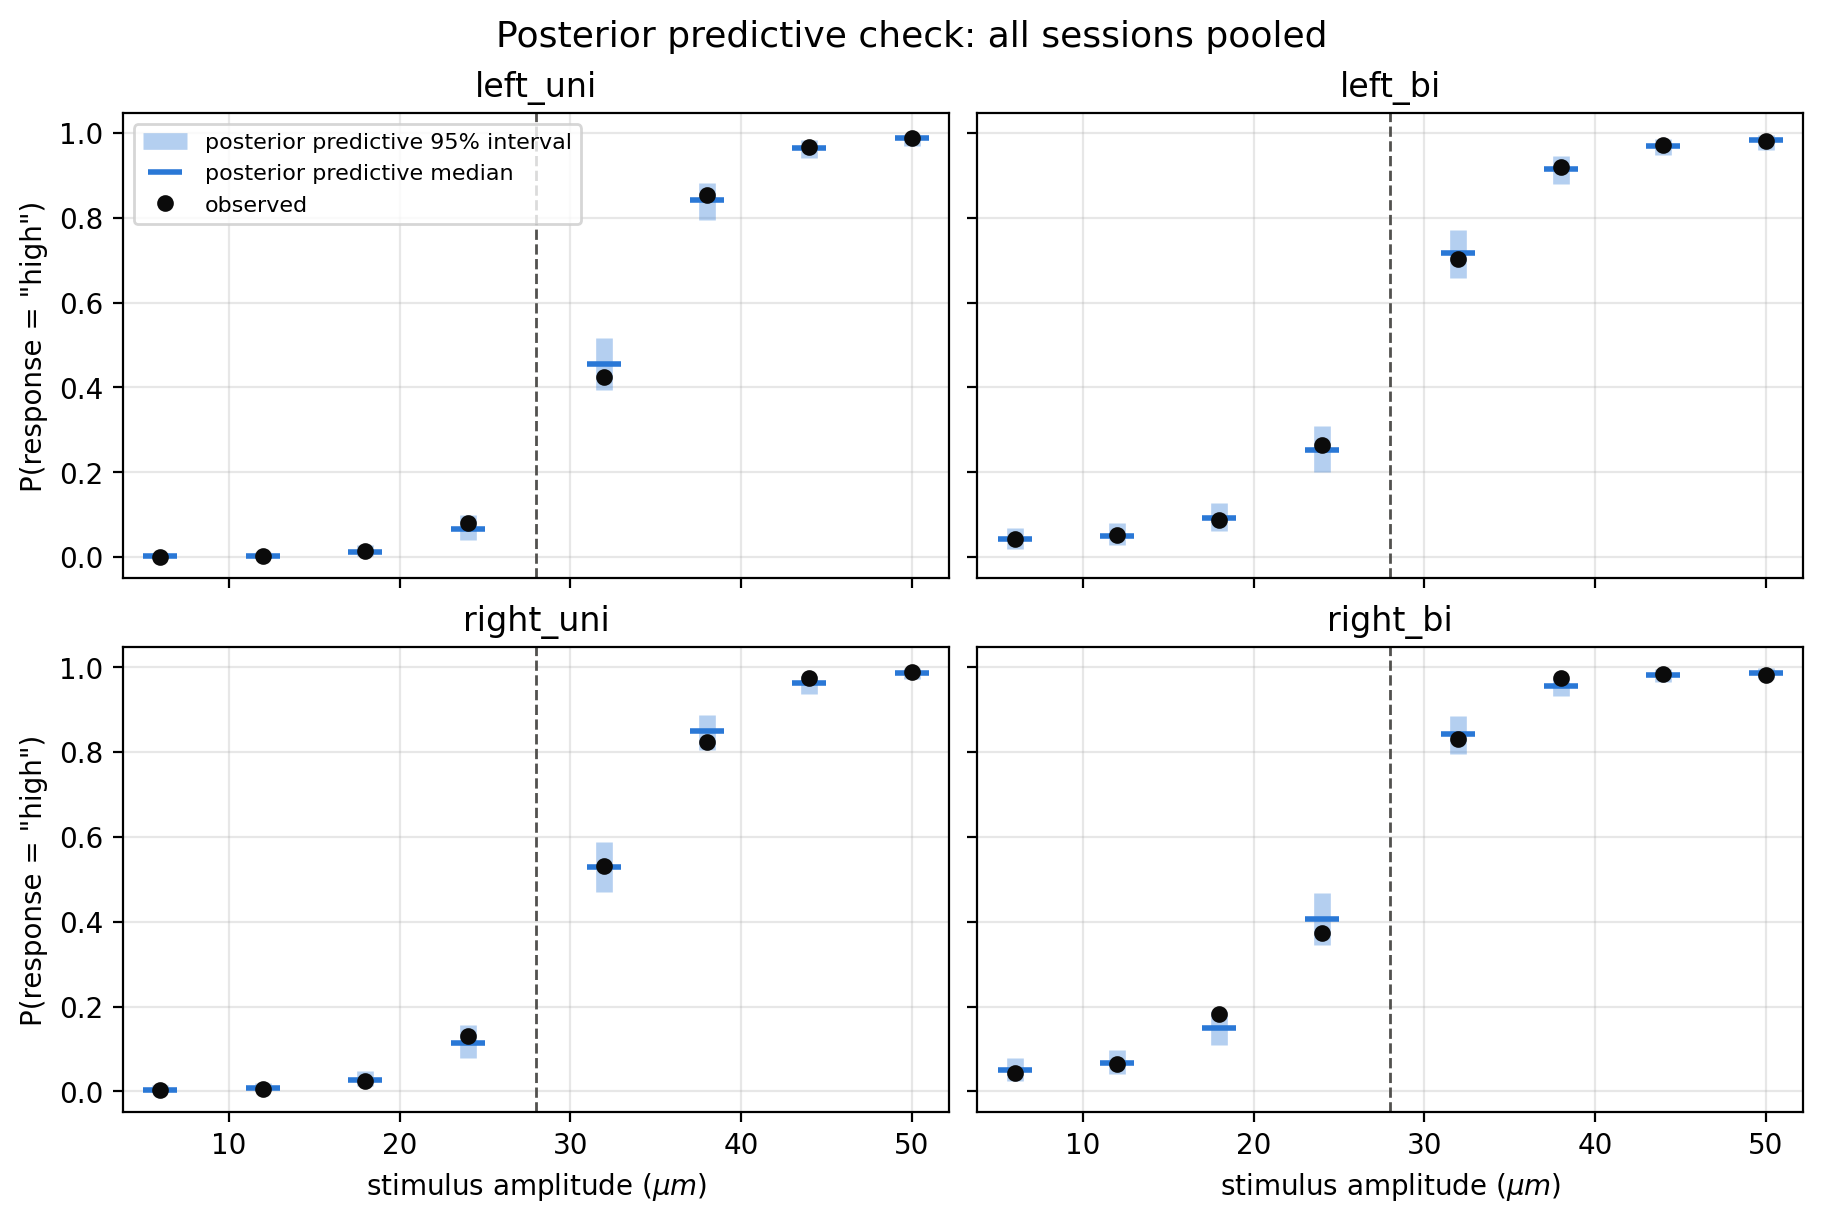
\includegraphics[width=0.85\textwidth]{ppc_pooled_by_stimulus.png}
\caption{Observed proportion of ``high'' responses at each amplitude, pooled
over sessions (black), against the posterior predictive median and 95\%
interval (blue). The dashed line is the trained threshold.}
\label{fig:ppc}
\end{figure}

Pooled over sessions, all 32 group-by-amplitude proportions lie inside their
95\% posterior predictive intervals (Figure~\ref{fig:ppc}): one curve per
group describes the pooled data well.

\begin{figure}[H]
\centering
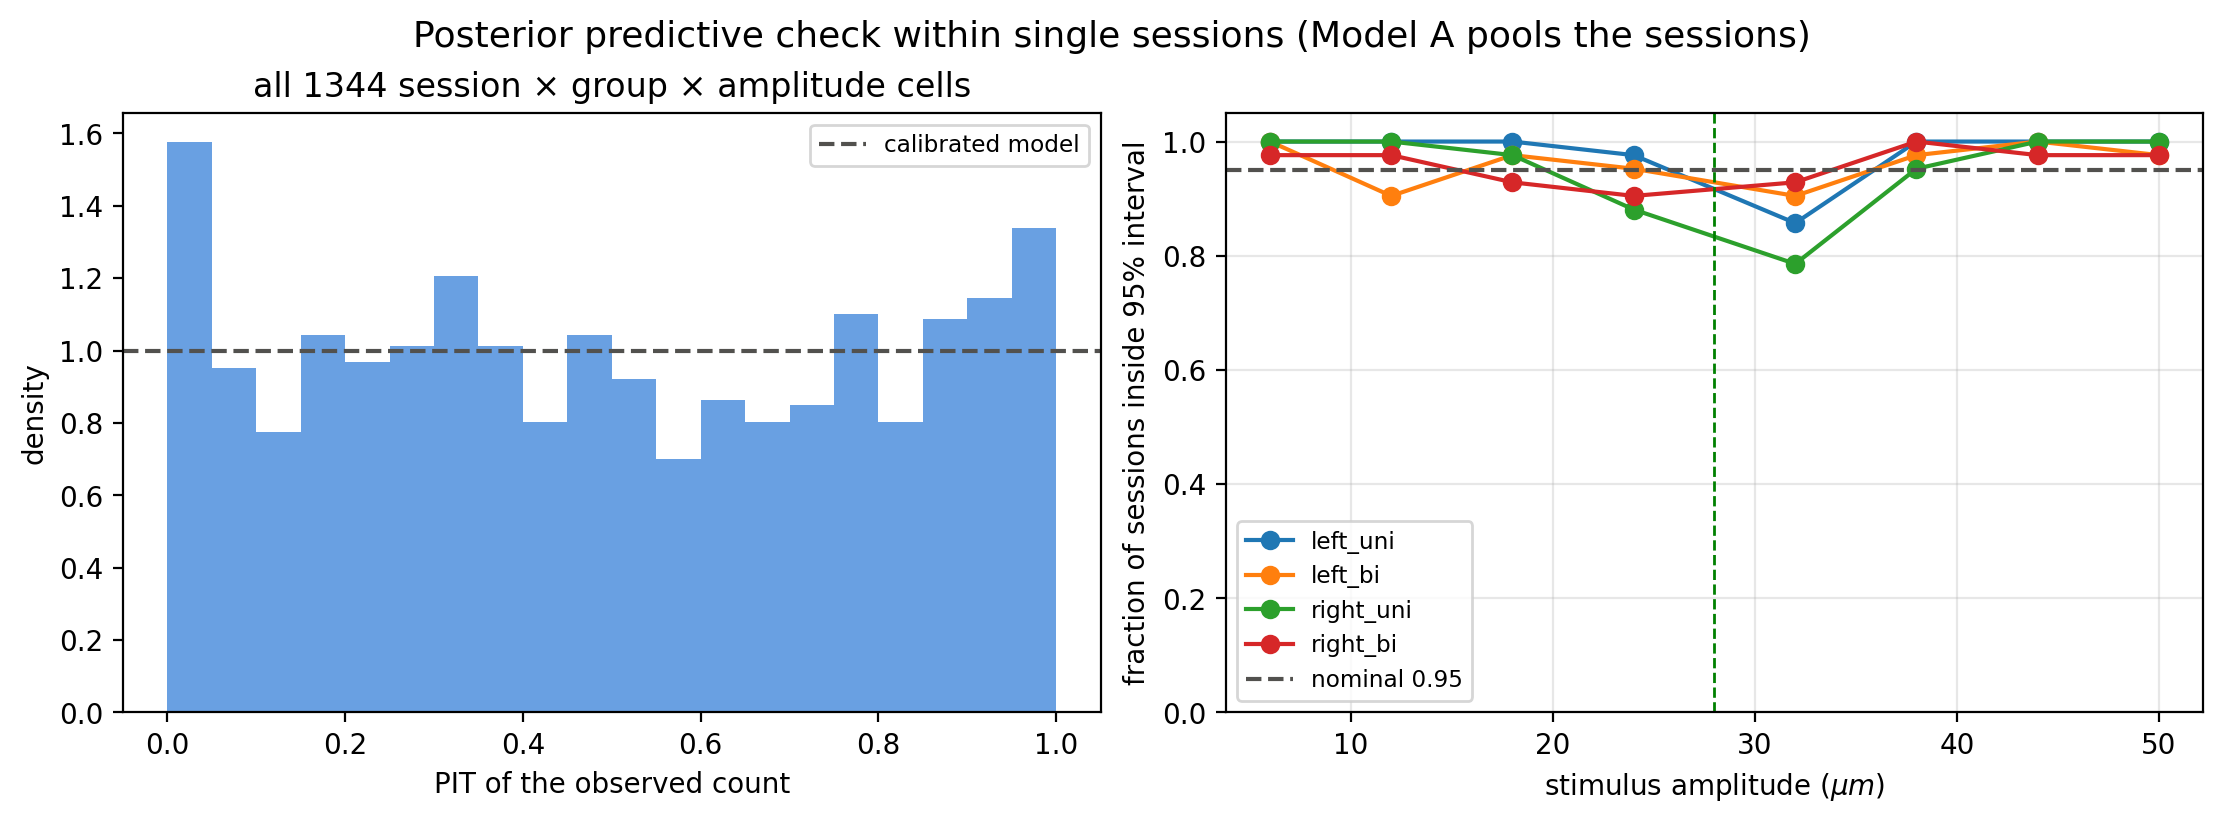
\includegraphics[width=\textwidth]{ppc_session_cells.png}
\caption{Posterior predictive check within single sessions. Left: PIT values of
the observed number of ``high'' responses in each session $\times$ group
$\times$ amplitude cell (flat at 1 for a calibrated model). Right: fraction of
the 42 sessions whose observed count lies inside its 95\% predictive interval,
by group and amplitude.}
\label{fig:ppc_sessions}
\end{figure}

Within single sessions the picture is different (Figure~\ref{fig:ppc_sessions}).
Model A predicts the same curve in every session, so it treats the variation
between sessions as if it were trial noise. Overall, 1{,}293 of the 1{,}344
session $\times$ group $\times$ amplitude cells (96.2\%) lie inside their 95\%
intervals, close to nominal, but 4.5\% of the PIT values are below 0.025 and
4.0\% above 0.975, against 2.5\% each for a calibrated model: the session counts
vary more than Model A predicts. The excess is concentrated at 32 $\mu m$, the
level just above the threshold, where the curve is steepest and a small shift
of a session's PSE changes the response rate most: there only 79\% (right\_uni)
and 86\% (left\_uni) of sessions lie inside their intervals. The sessions' PSEs
differ, which a single curve per group cannot represent.

\subsection{Leave-one-out cross-validation}

Model A has $\text{elpd}_\text{loo} = -3344.0$ (SE 64.5) with
$p_\text{loo} = 13.4$, close to its 16 parameters, and every Pareto $k$ is at most
0.07, so the PSIS-LOO estimate is reliable. It is saved with the fit for comparison
with later models.

\section{Conclusions}

\begin{itemize}
  \item The fit is reliable: no divergences, $\hat{R} = 1.000$, bulk ESS above
        15{,}000, and the pooled data are reproduced at every amplitude.
  \item The distractor lowers the PSE by 4.2 (left) and 6.1 (right) $\mu m$ and
        raises $\gamma_h$ by about 0.04; it raises the left-hand JND by about
        0.8 $\mu m$.
  \item Model A ignores the variation between sessions, which is real: within
        single sessions the responses near the threshold vary more than Model A
        allows. Pooling curves whose PSEs differ from session to session gives a
        shallower curve than any single session has, so the pooled JNDs may mix
        the monkey's precision within a session with the drift of its PSE between
        sessions, and the HDIs describe only the sessions observed.
  \item Model A is a useful, fast summary of the pooled data. A model with a
        curve for every session is needed to separate within-session precision
        from between-session variation.
\end{itemize}

\appendix
\section{Further Figures}
\label{app:figs}

\begin{figure}[H]
\centering
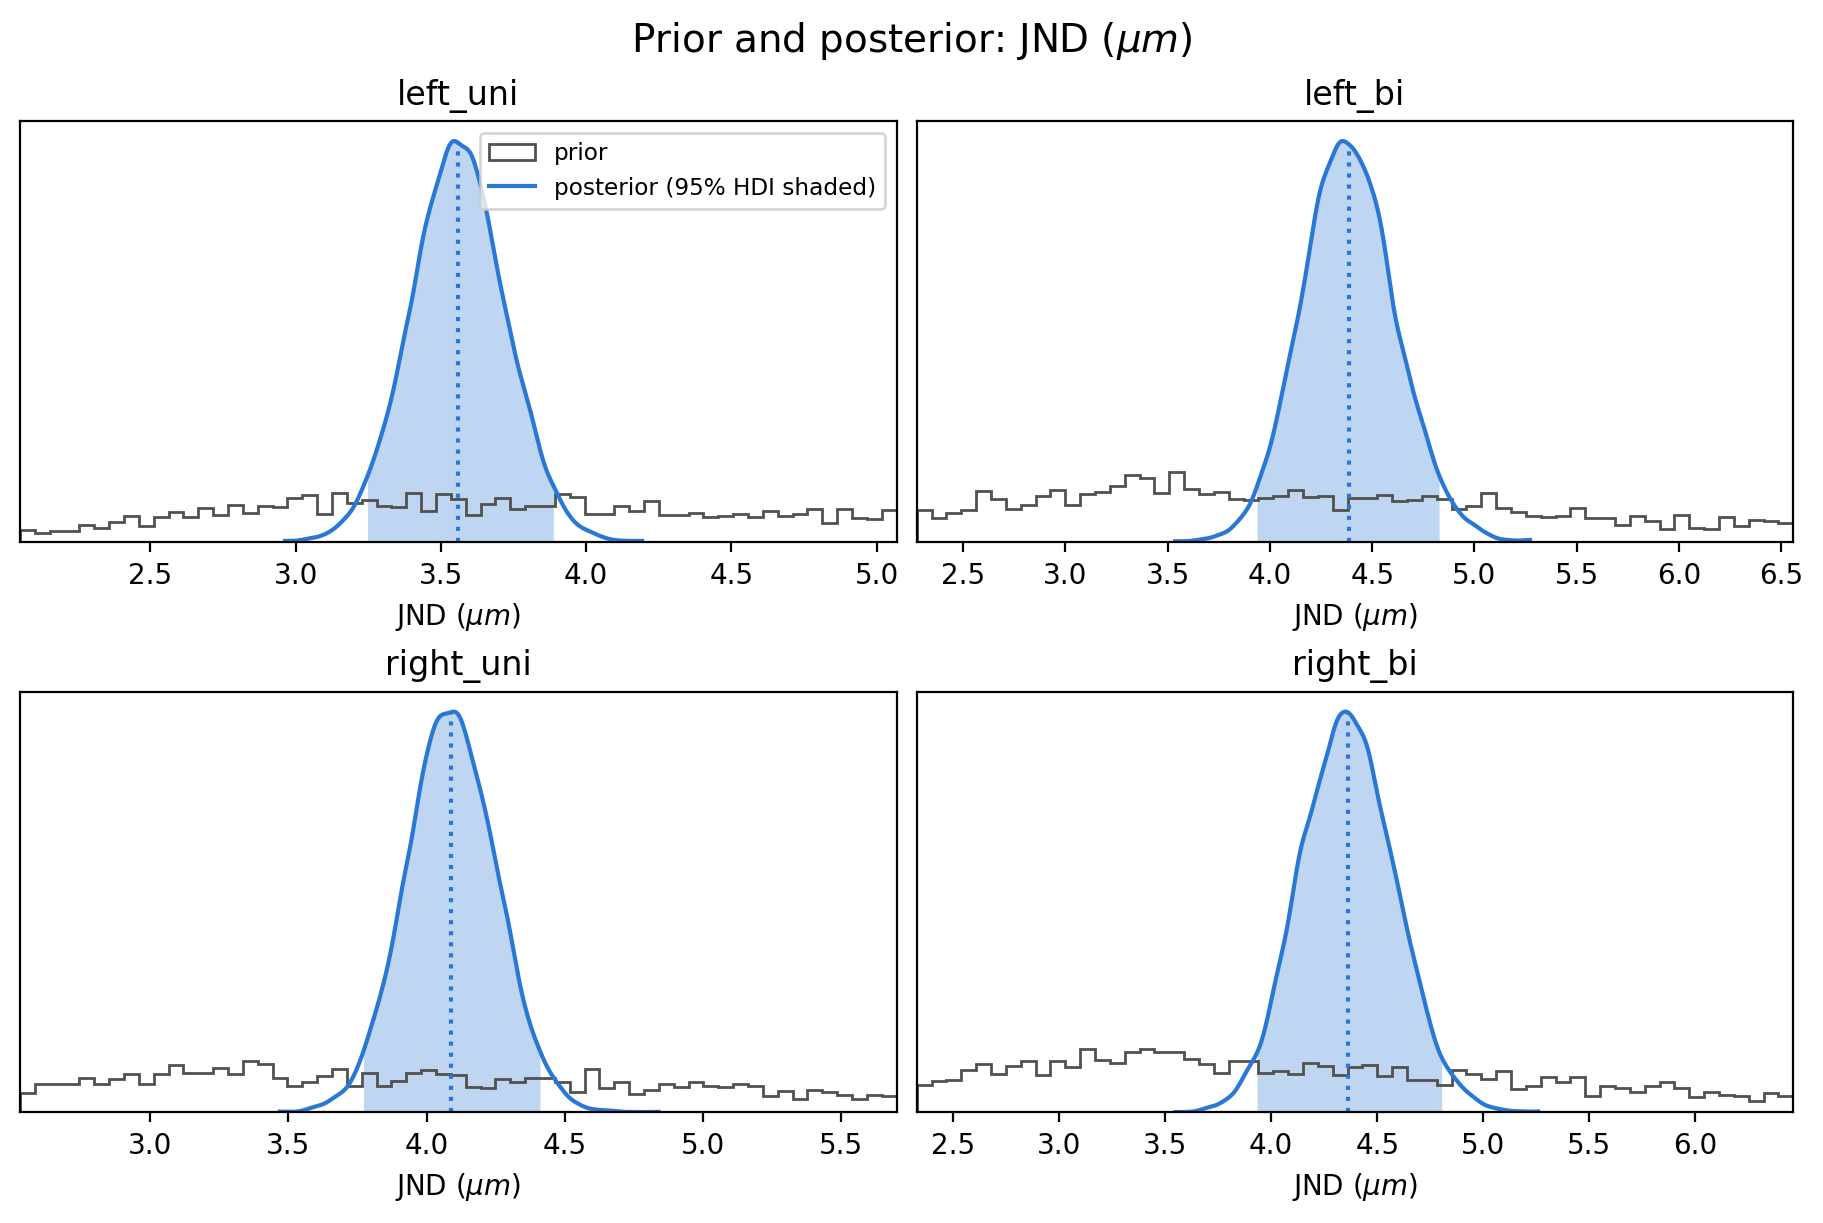
\includegraphics[width=0.8\textwidth]{prior_post_JND.png}
\caption{Prior (gray) and posterior (blue) of the JND.}
\end{figure}

\begin{figure}[H]
\centering
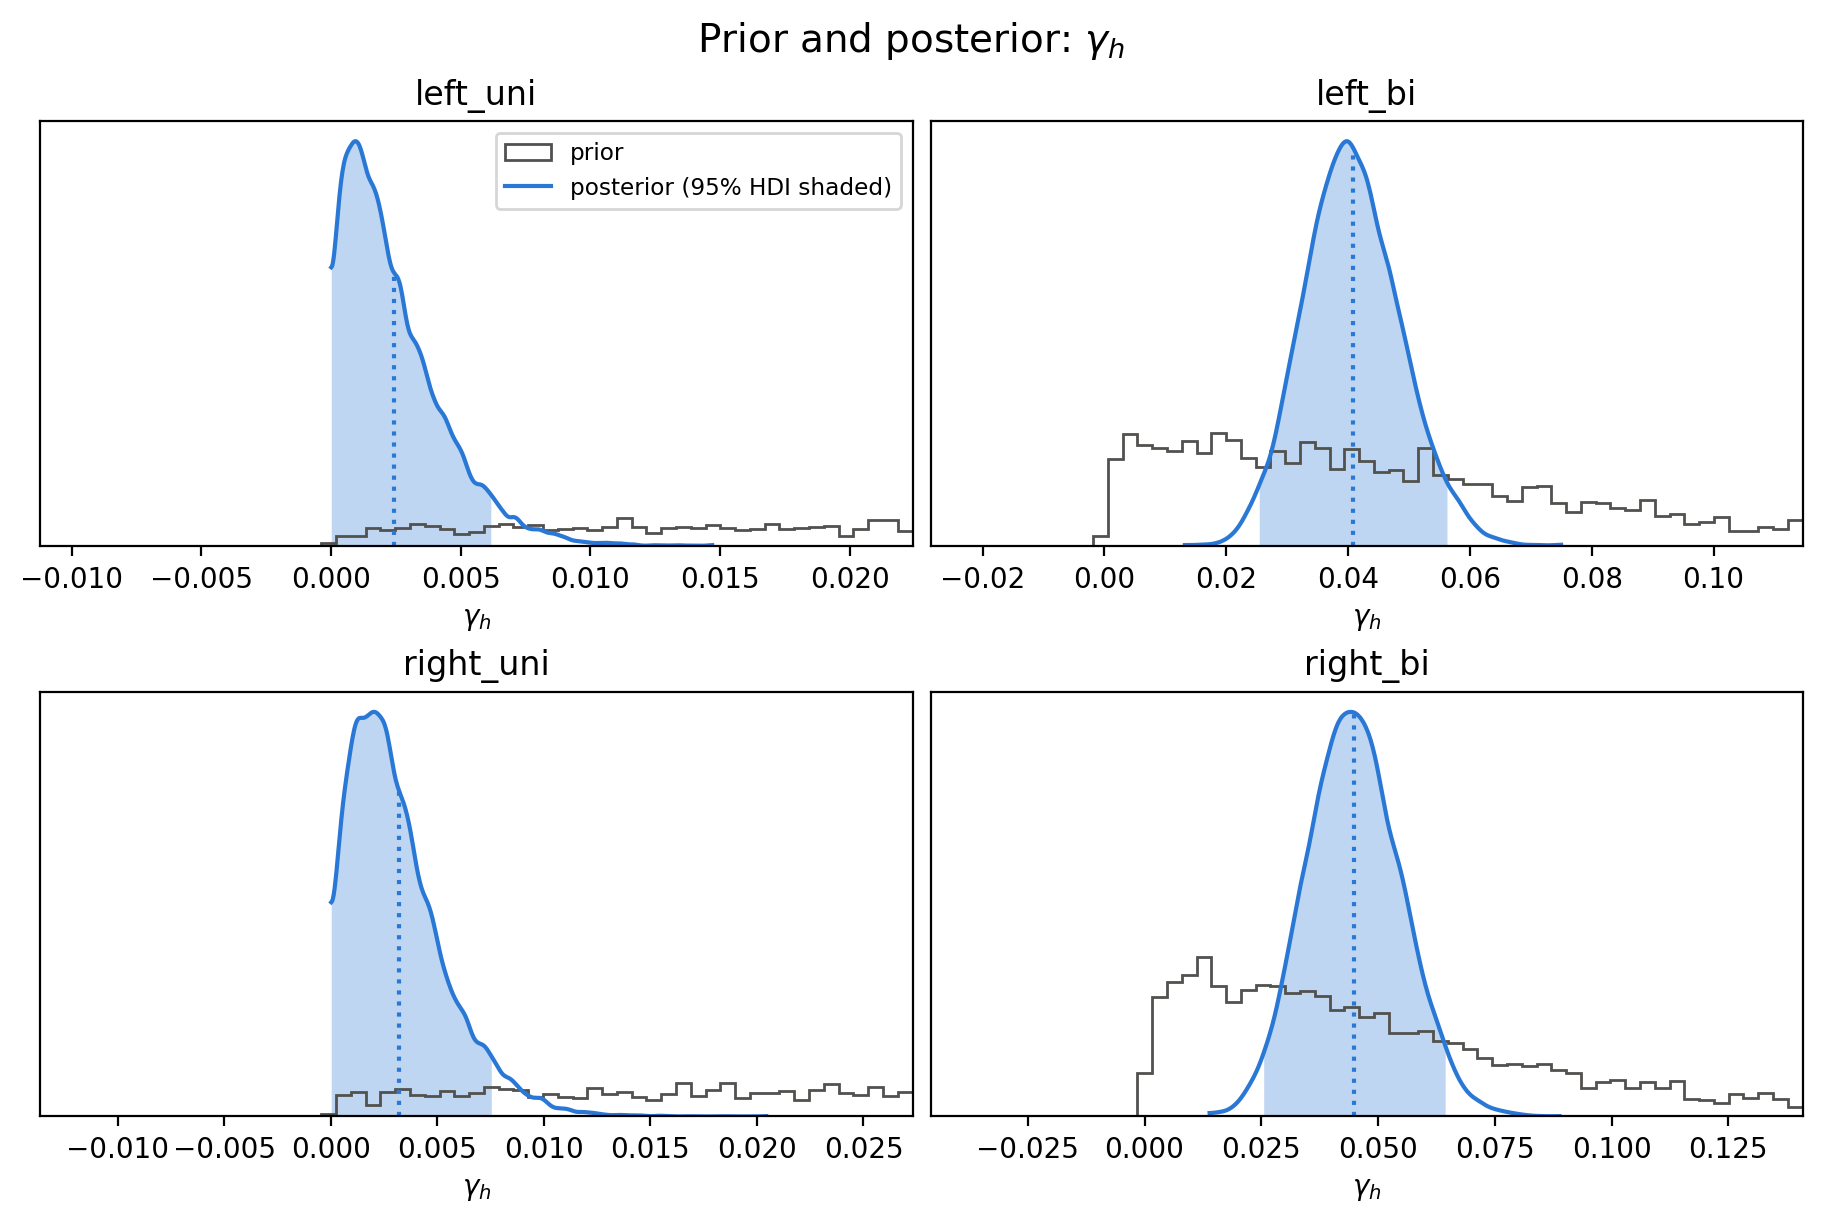
\includegraphics[width=0.8\textwidth]{prior_post_gamh.png}
\caption{Prior (gray) and posterior (blue) of $\gamma_h$.}
\end{figure}

\begin{figure}[H]
\centering
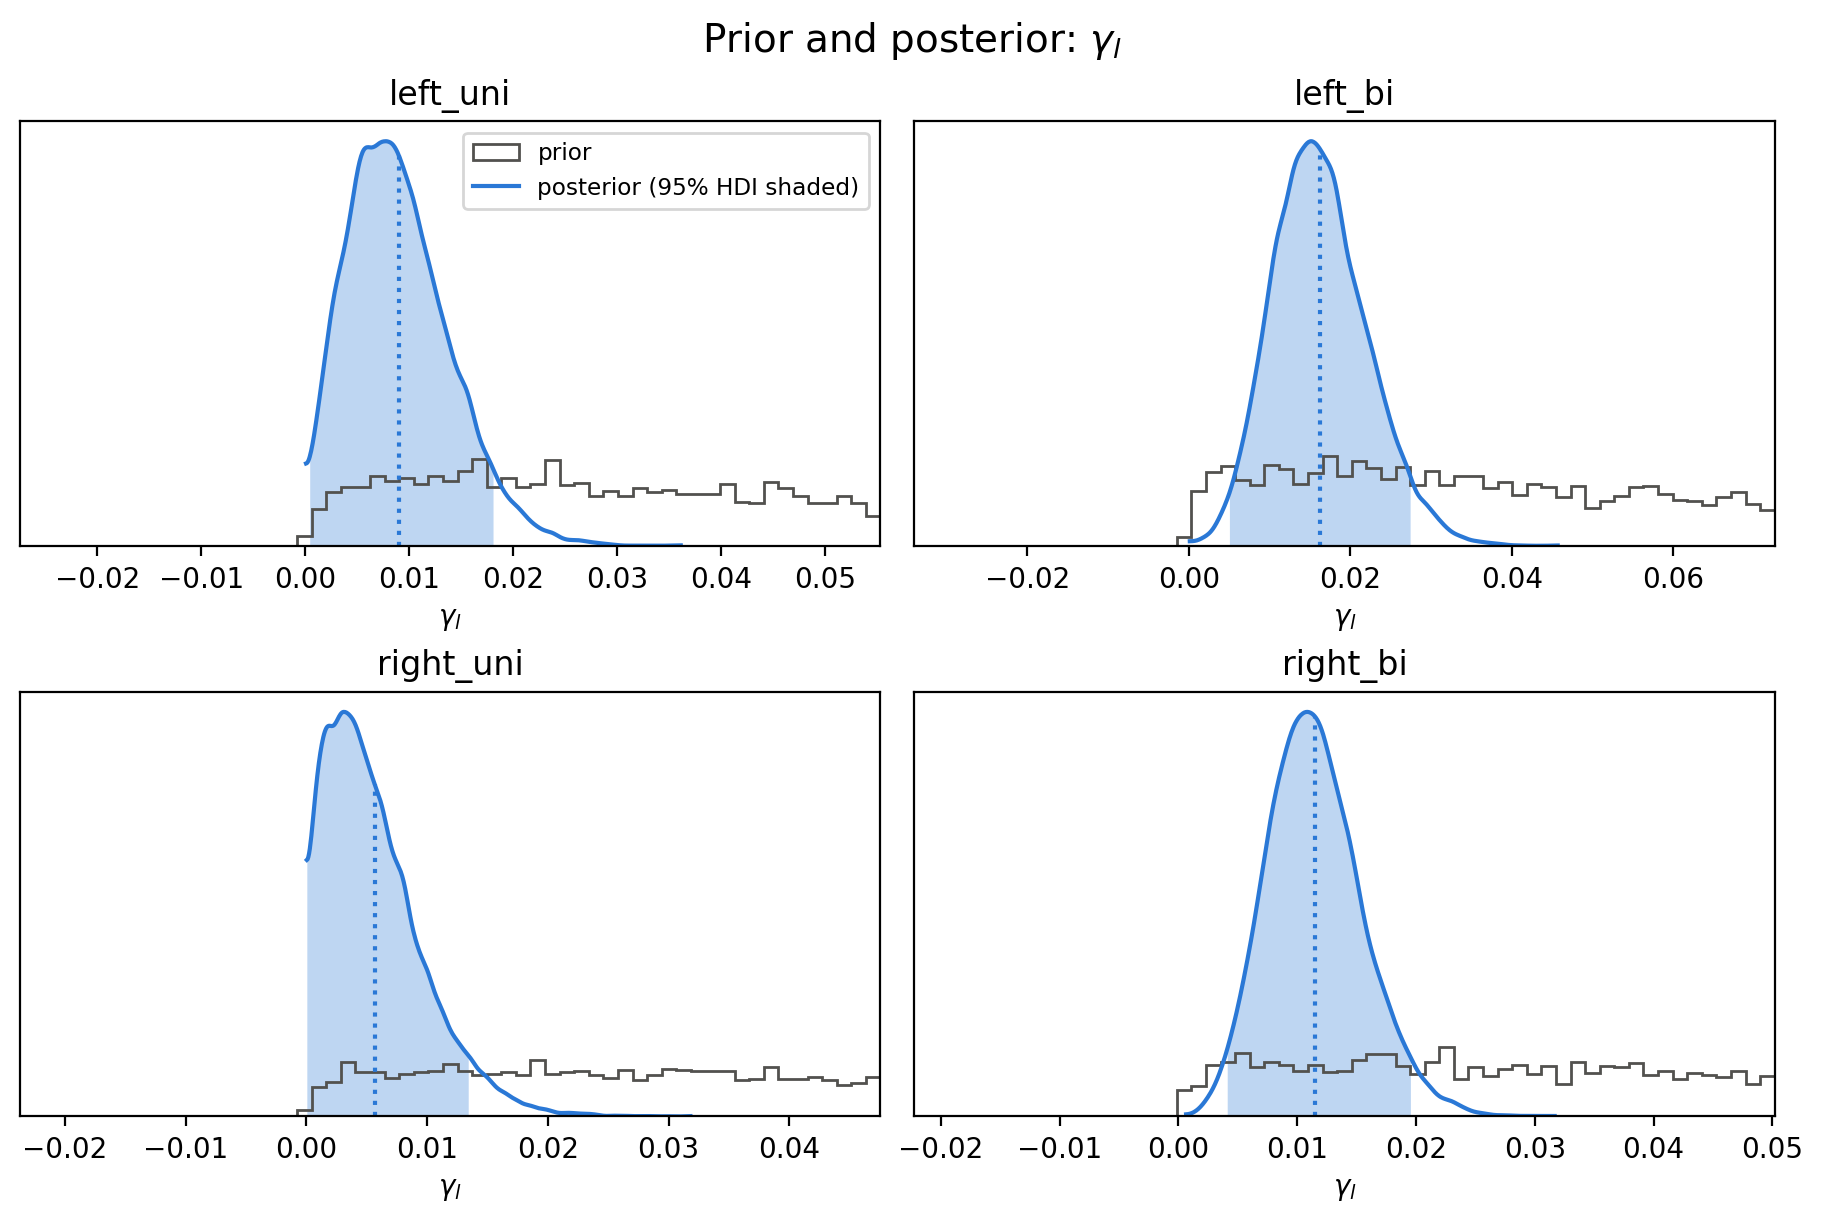
\includegraphics[width=0.8\textwidth]{prior_post_gaml.png}
\caption{Prior (gray) and posterior (blue) of $\gamma_l$.}
\end{figure}

\begin{figure}[H]
\centering
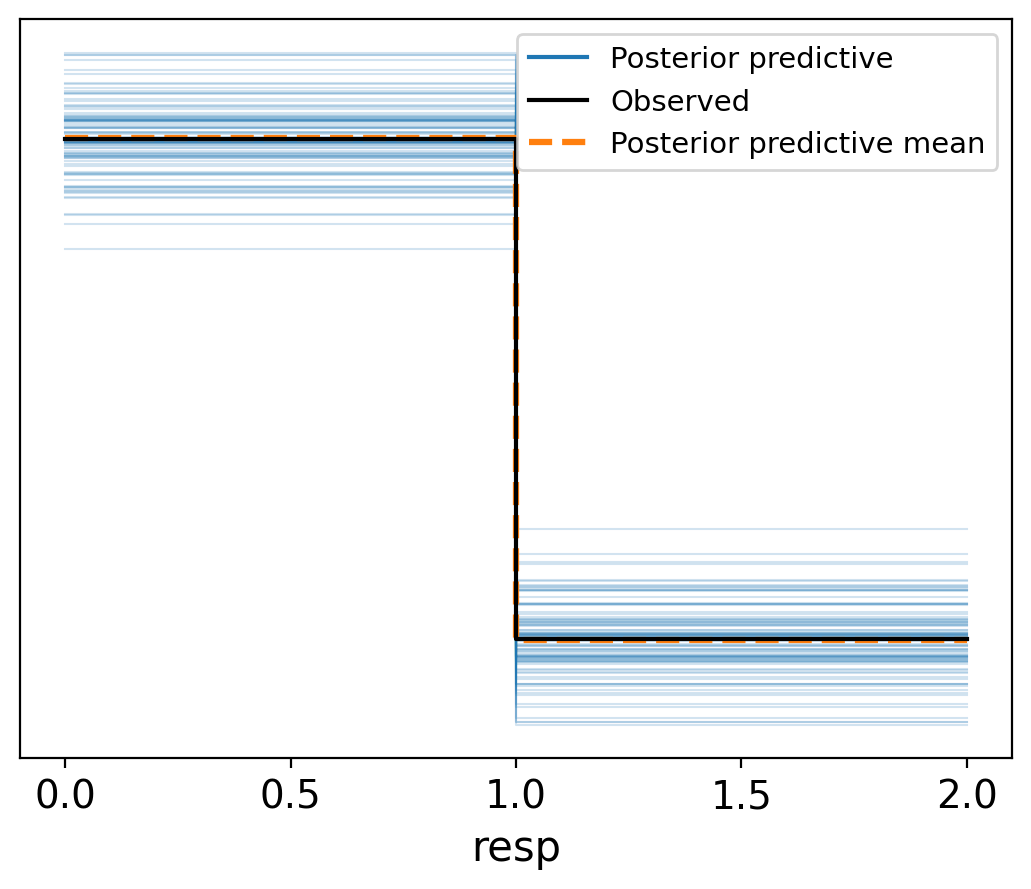
\includegraphics[width=0.55\textwidth]{ppc_arviz_resp.png}
\caption{ArviZ posterior predictive check of the responses (0 = ``low'',
1 = ``high''), pooled over all trials: observed (black), 100 posterior
predictive draws (blue) and their mean (orange dashed).}
\end{figure}

\begin{figure}[H]
\centering
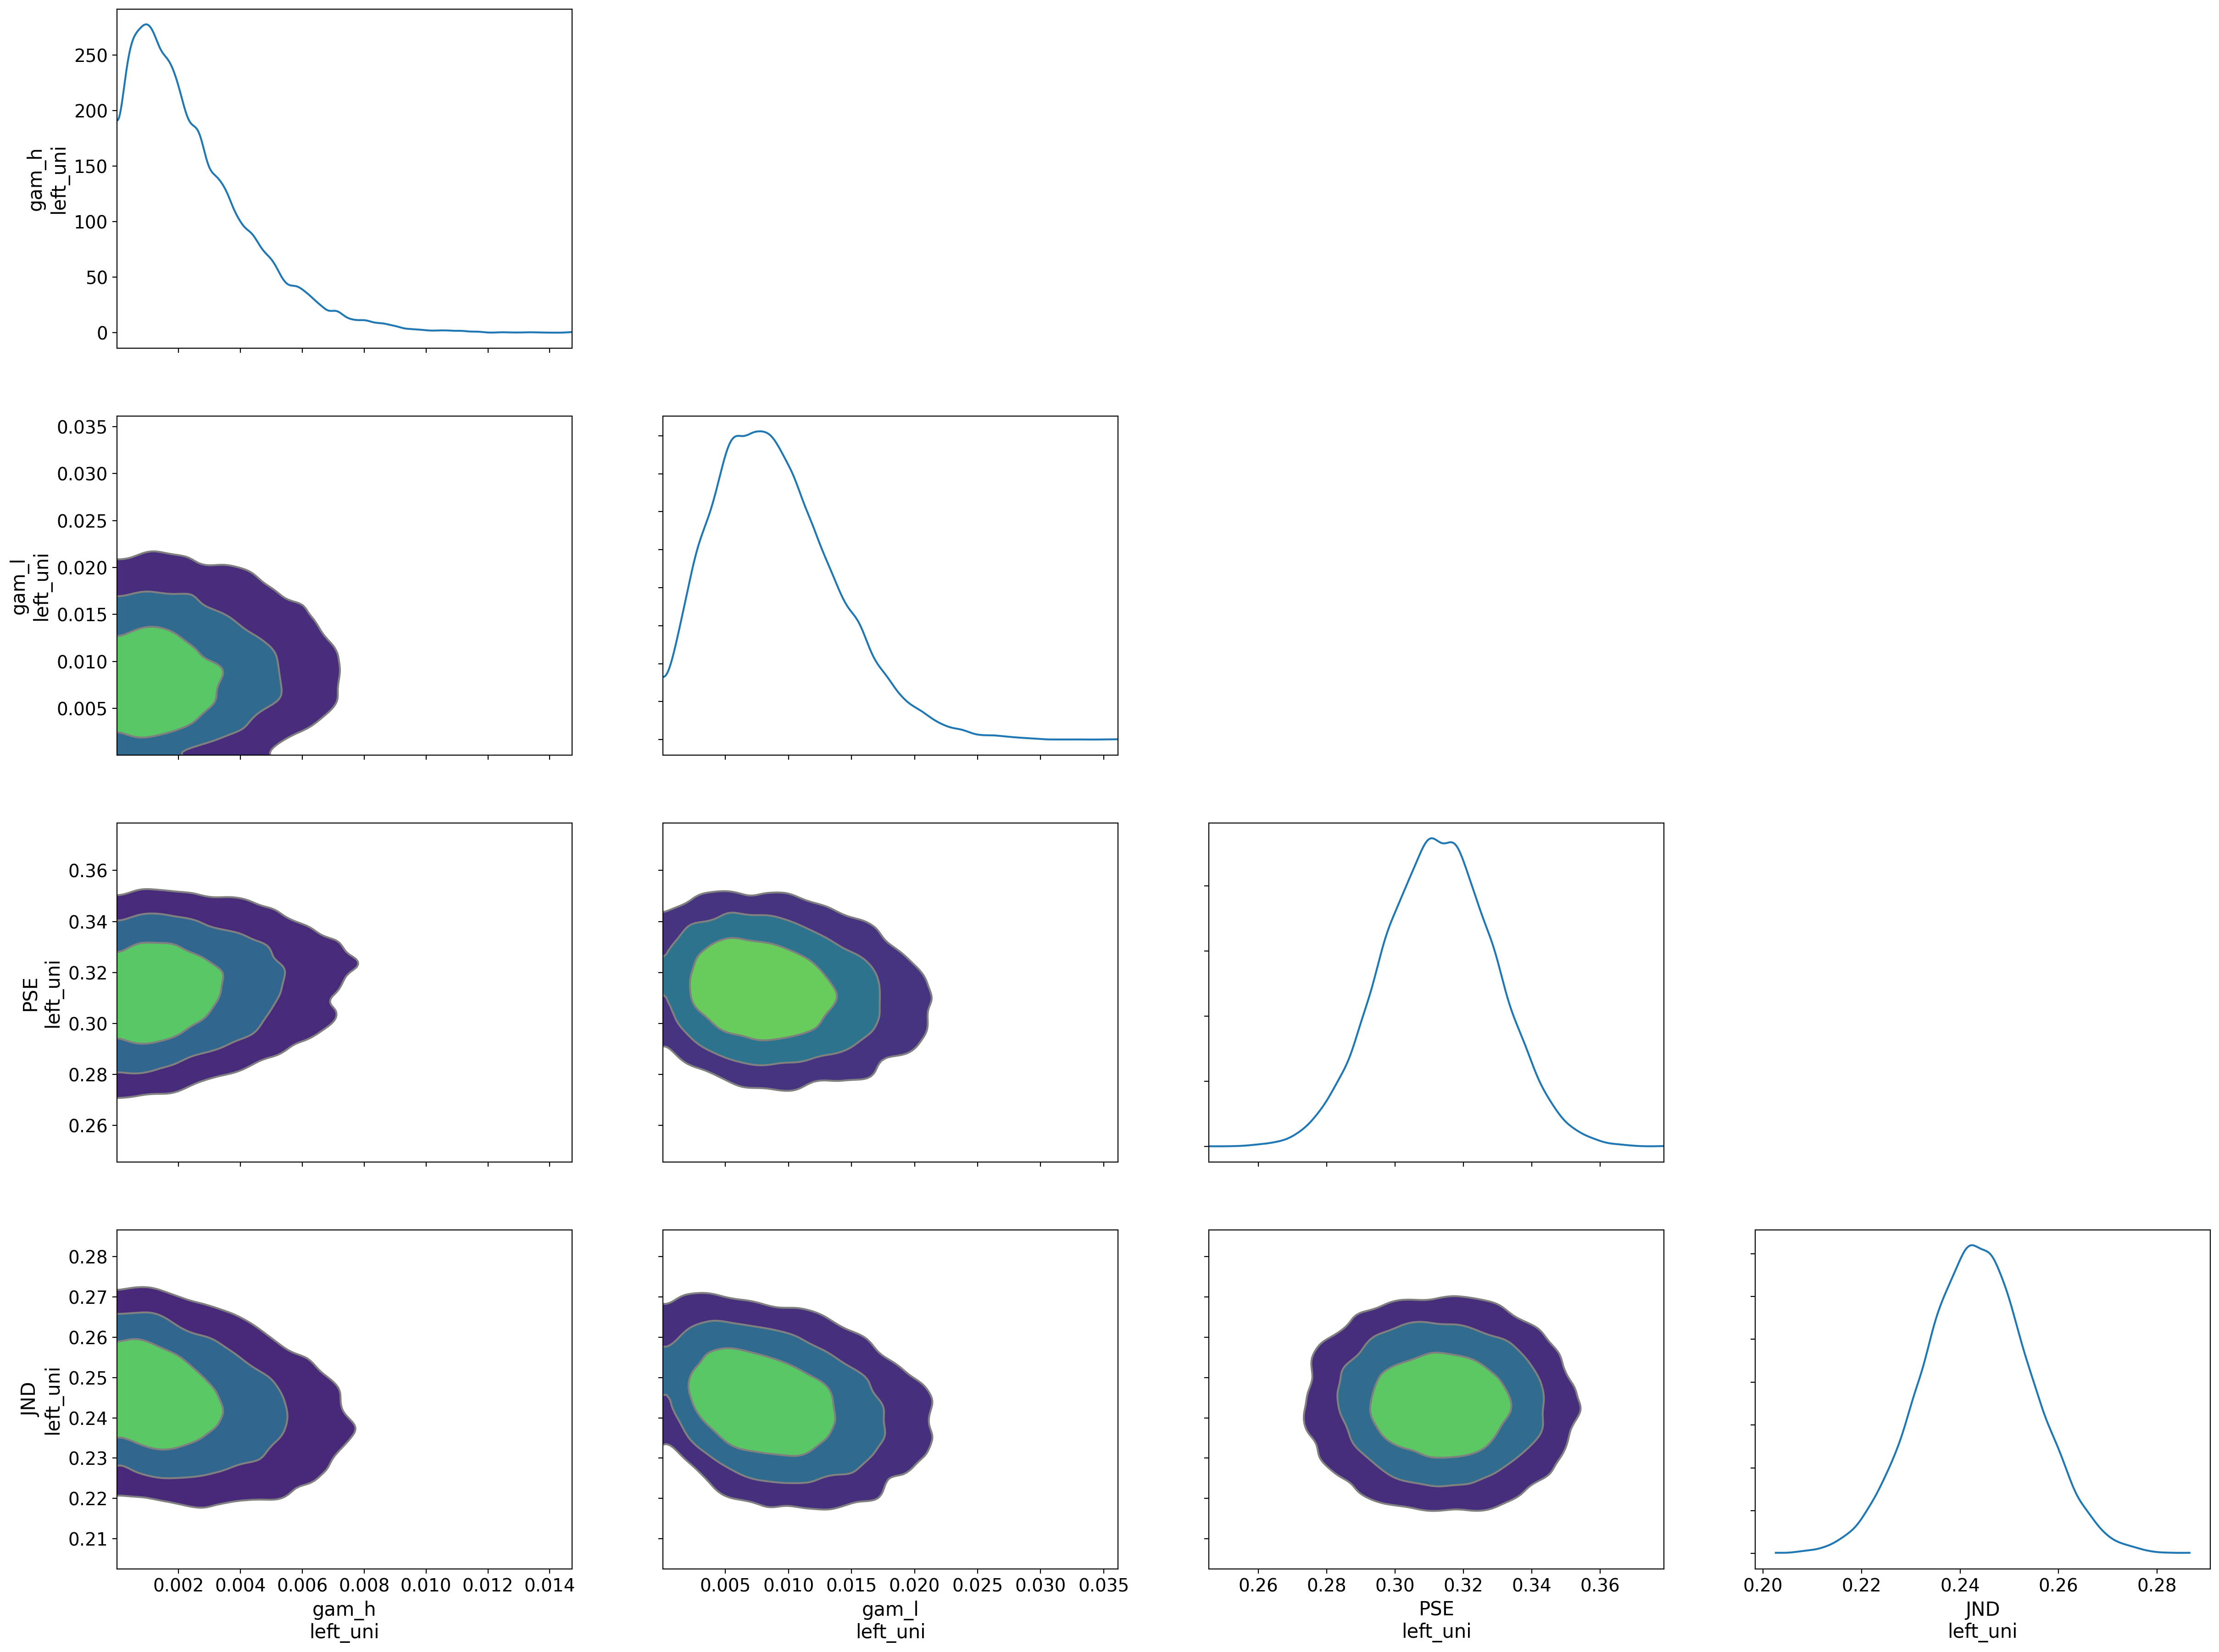
\includegraphics[width=0.48\textwidth]{pair_left_uni.png}\hfill
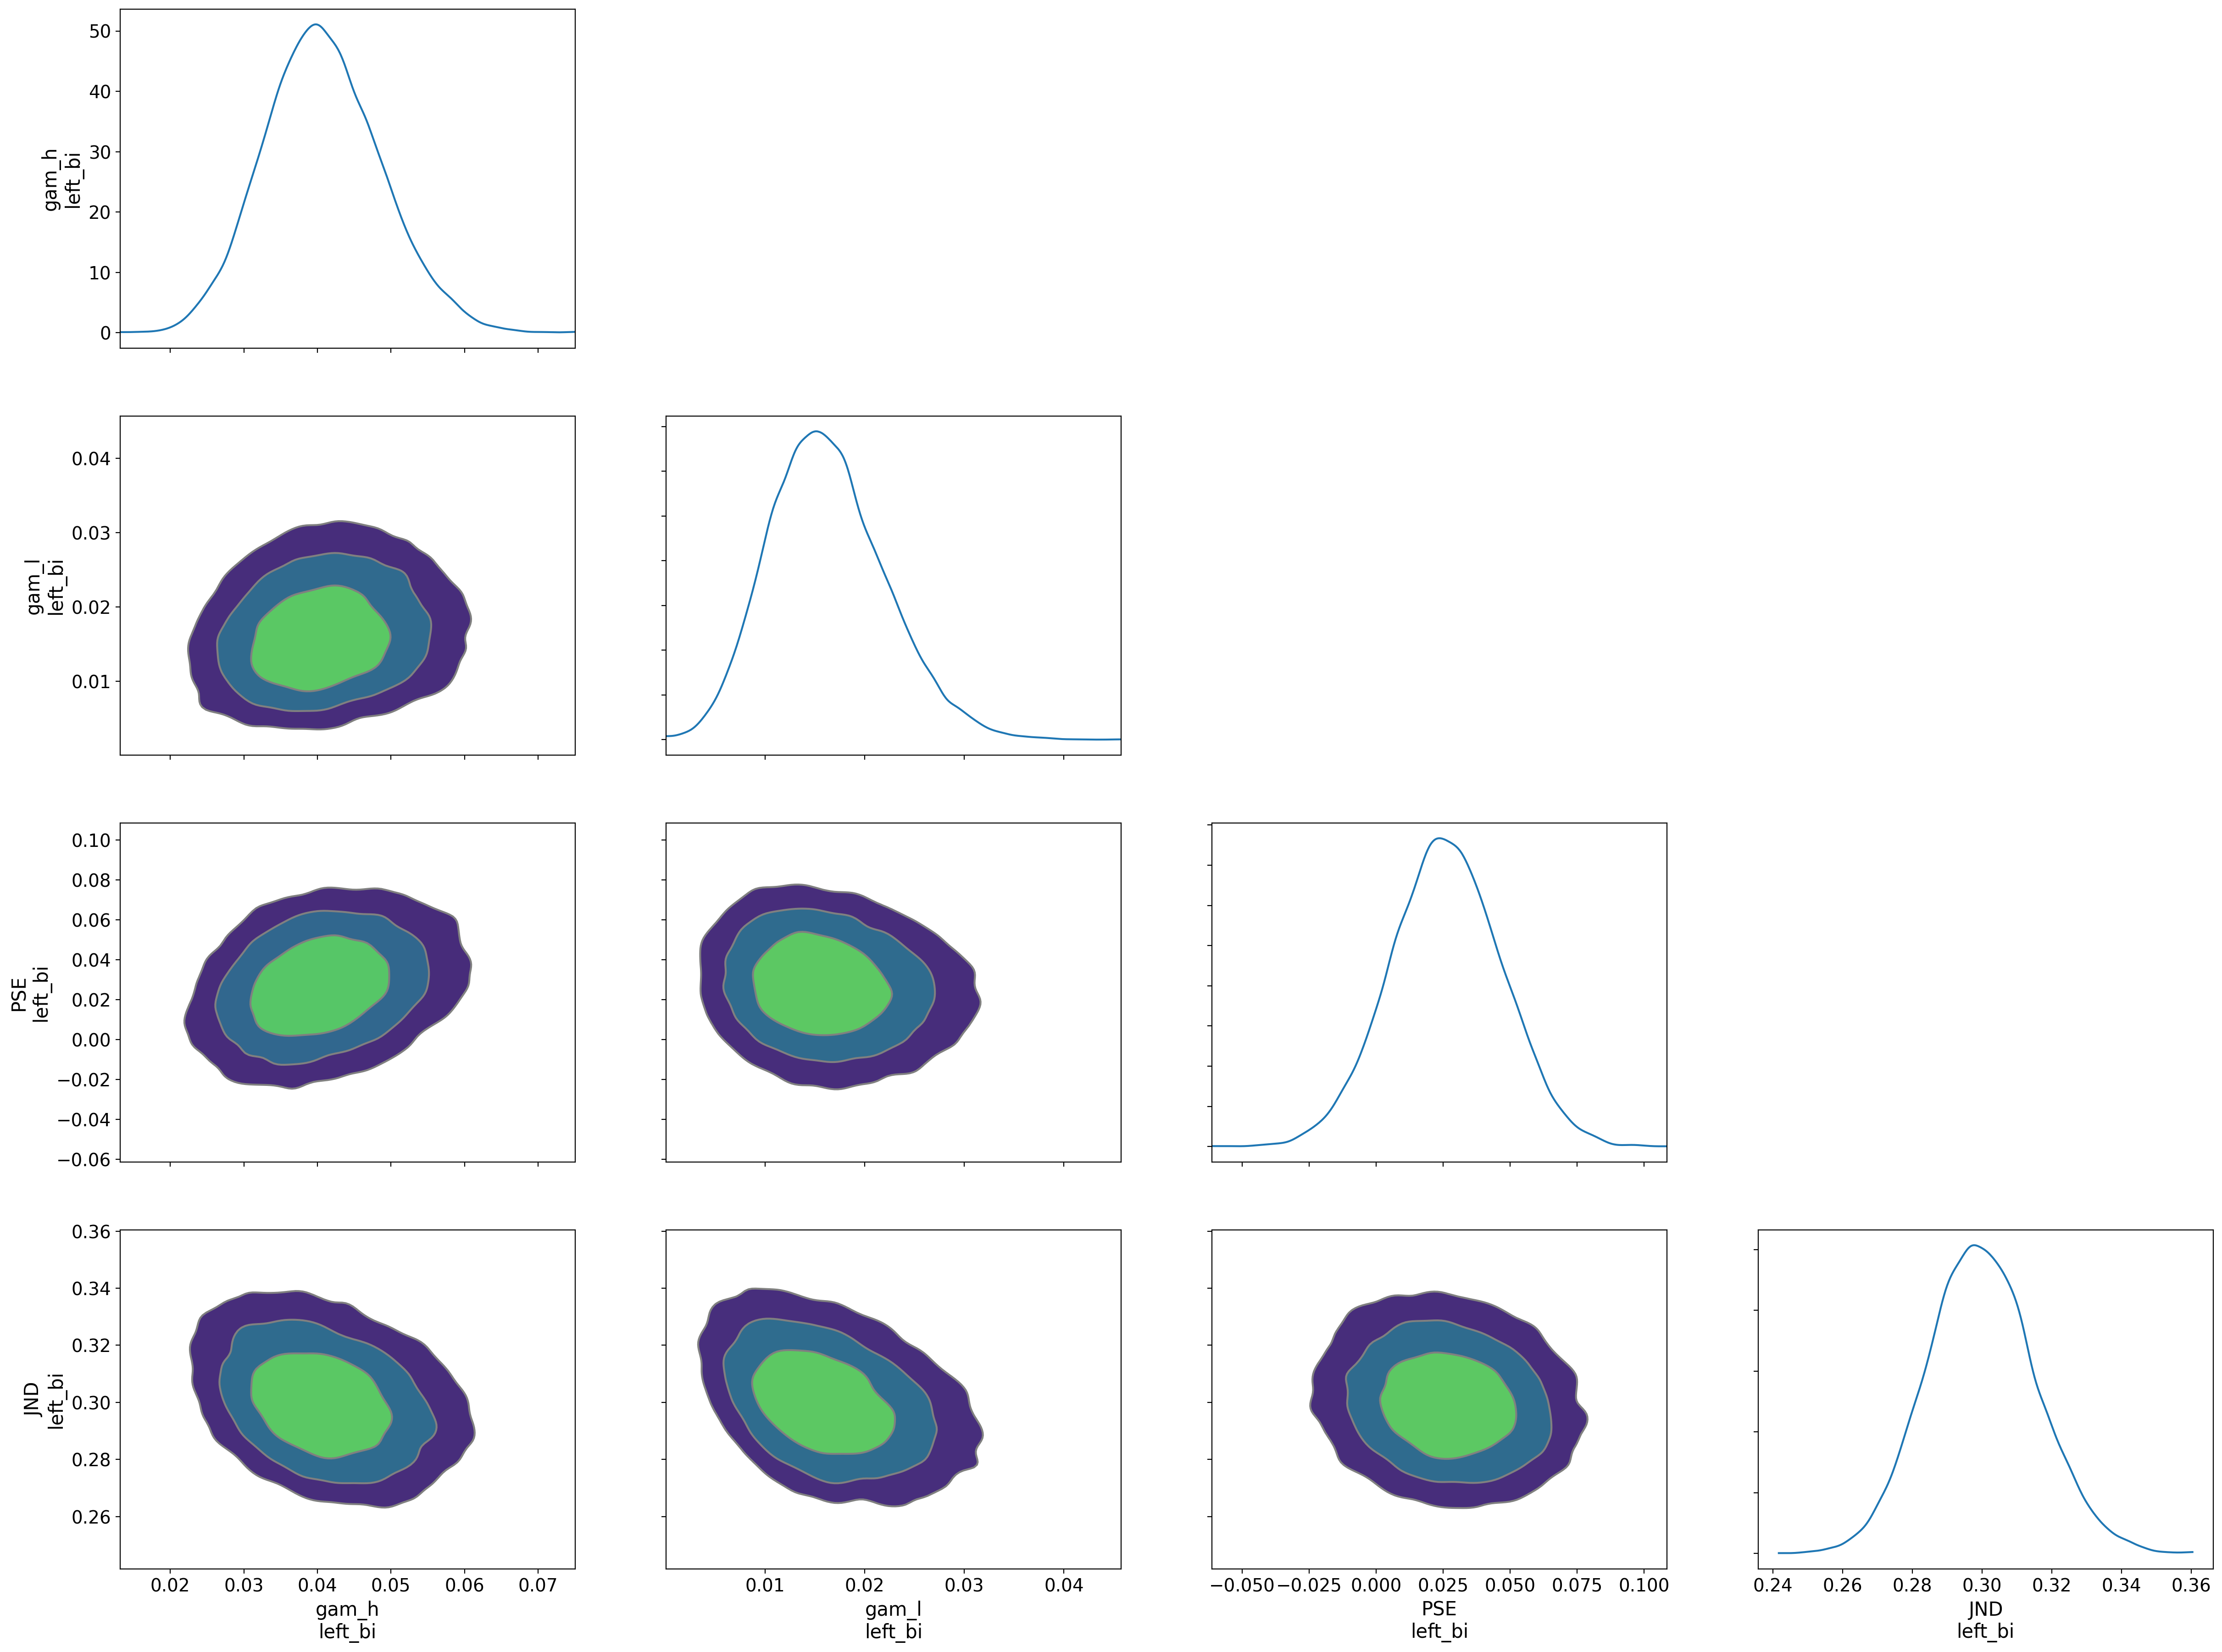
\includegraphics[width=0.48\textwidth]{pair_left_bi.png}

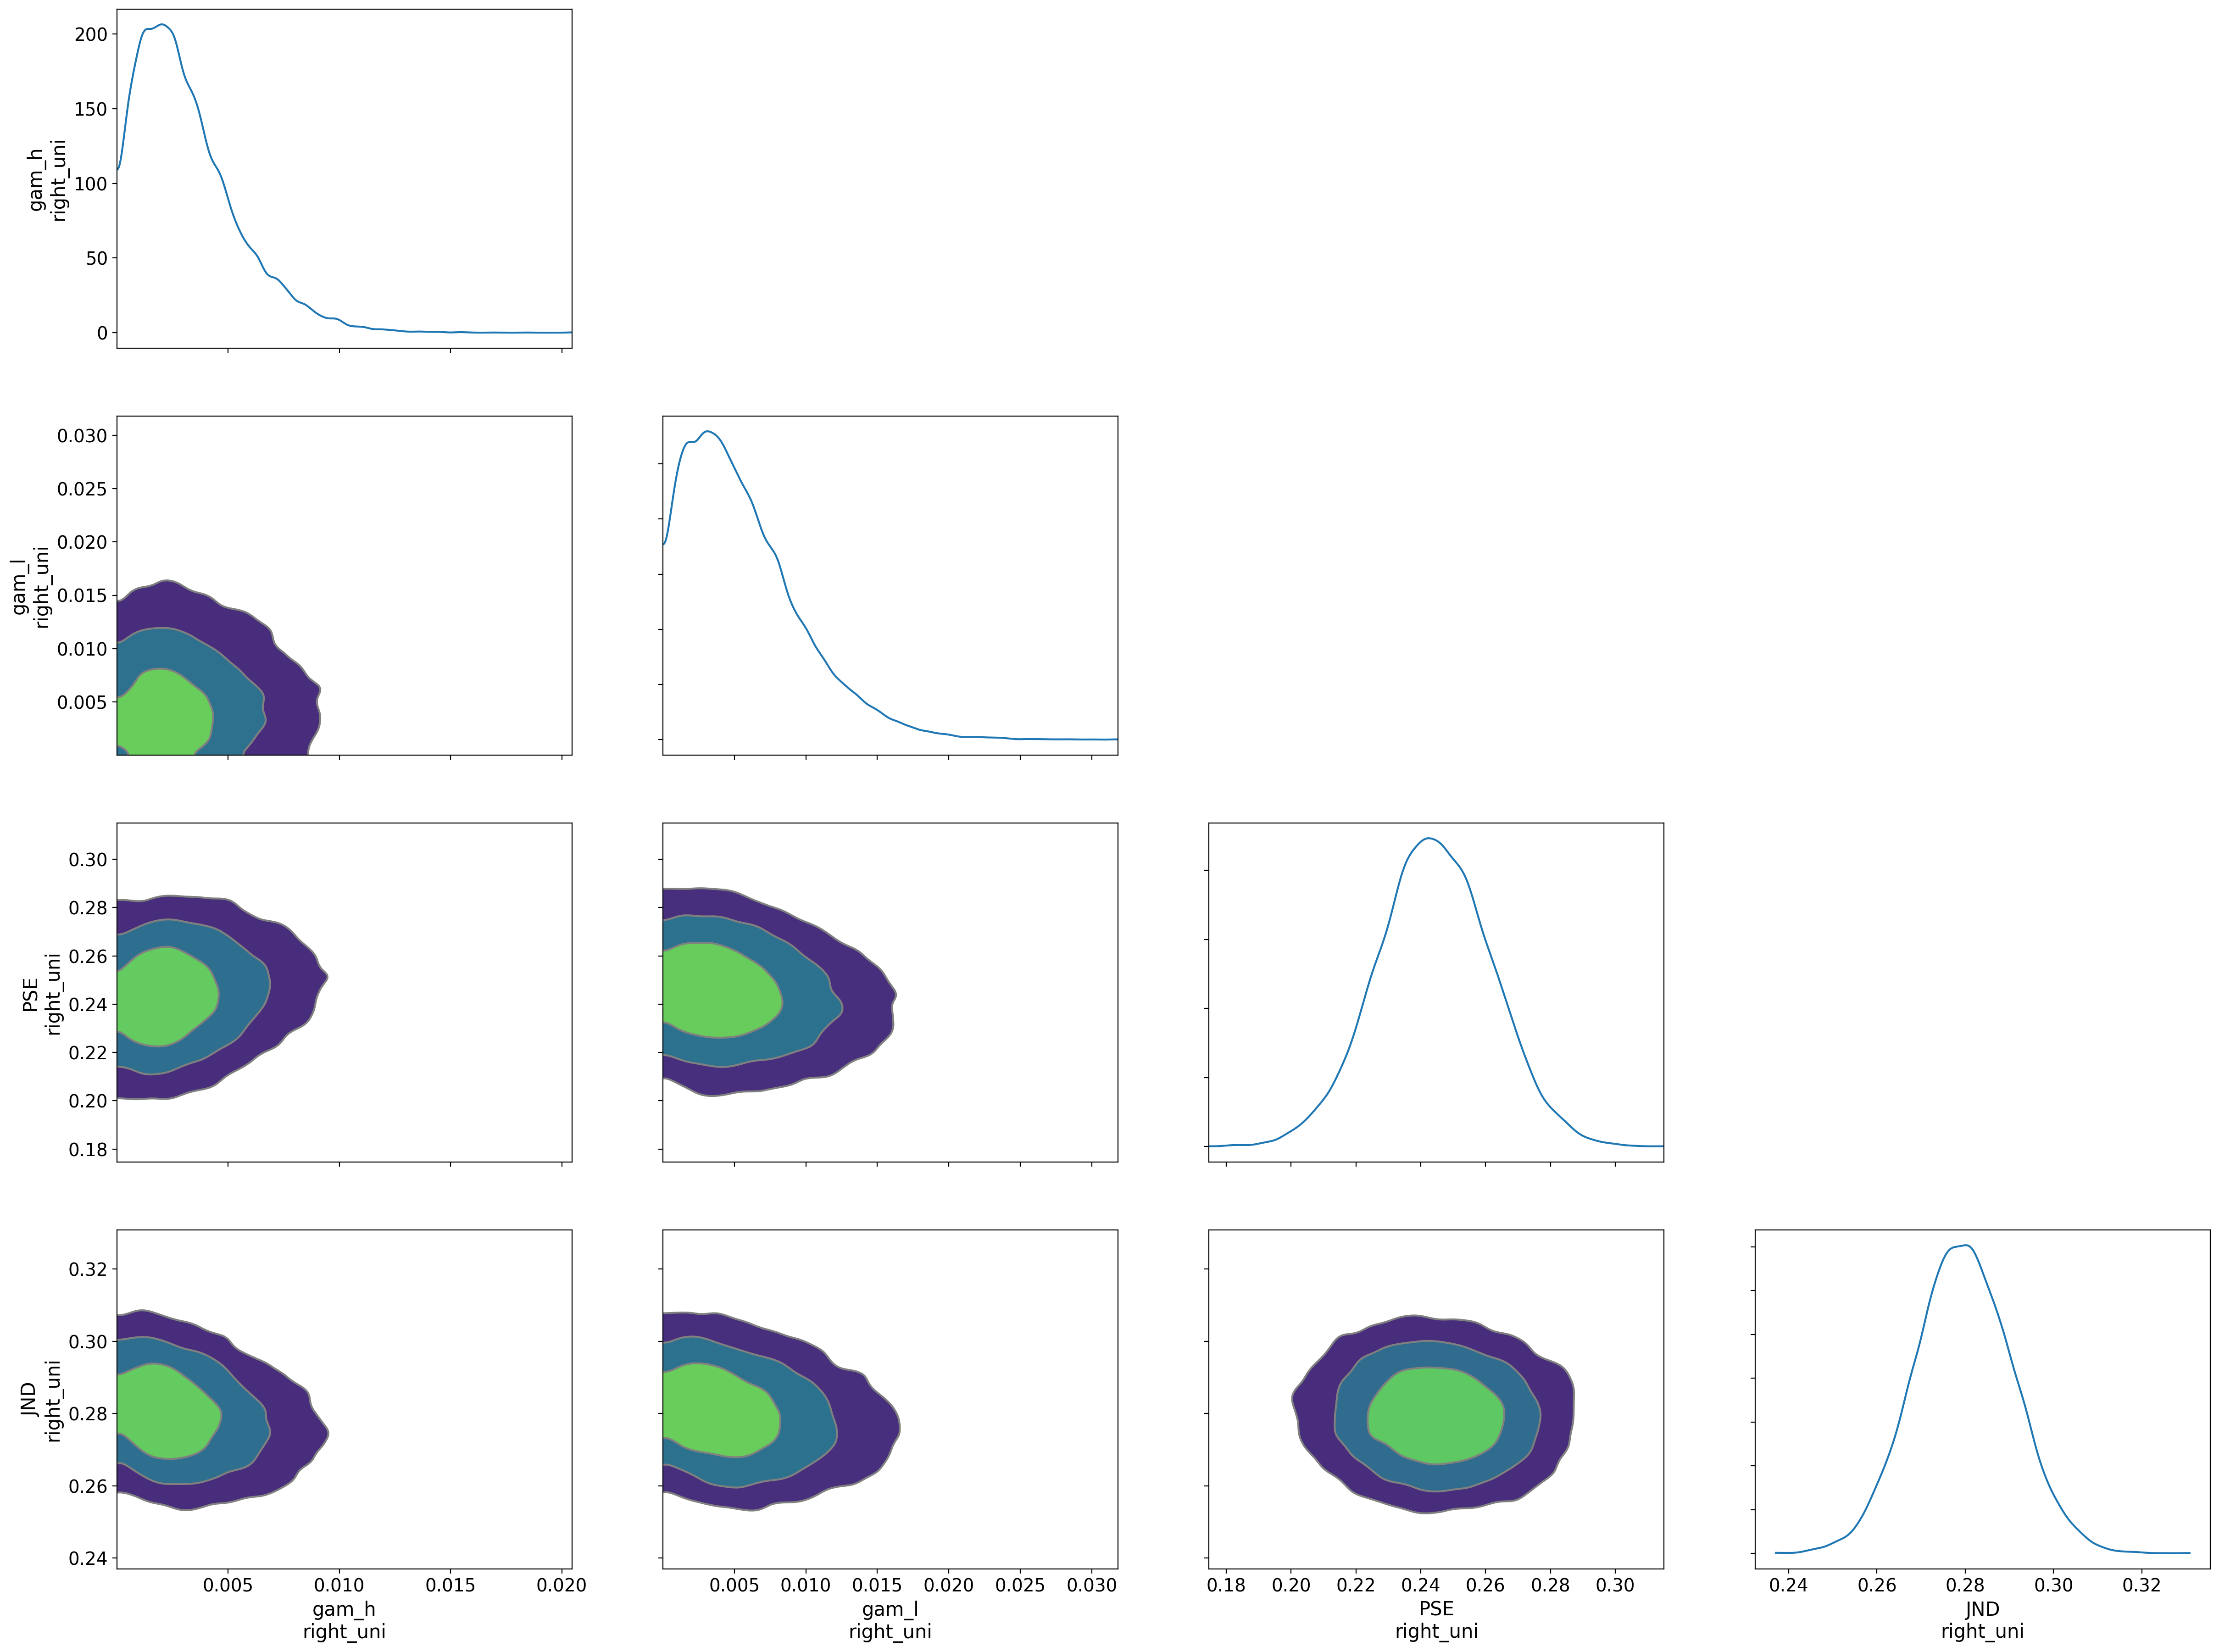
\includegraphics[width=0.48\textwidth]{pair_right_uni.png}\hfill
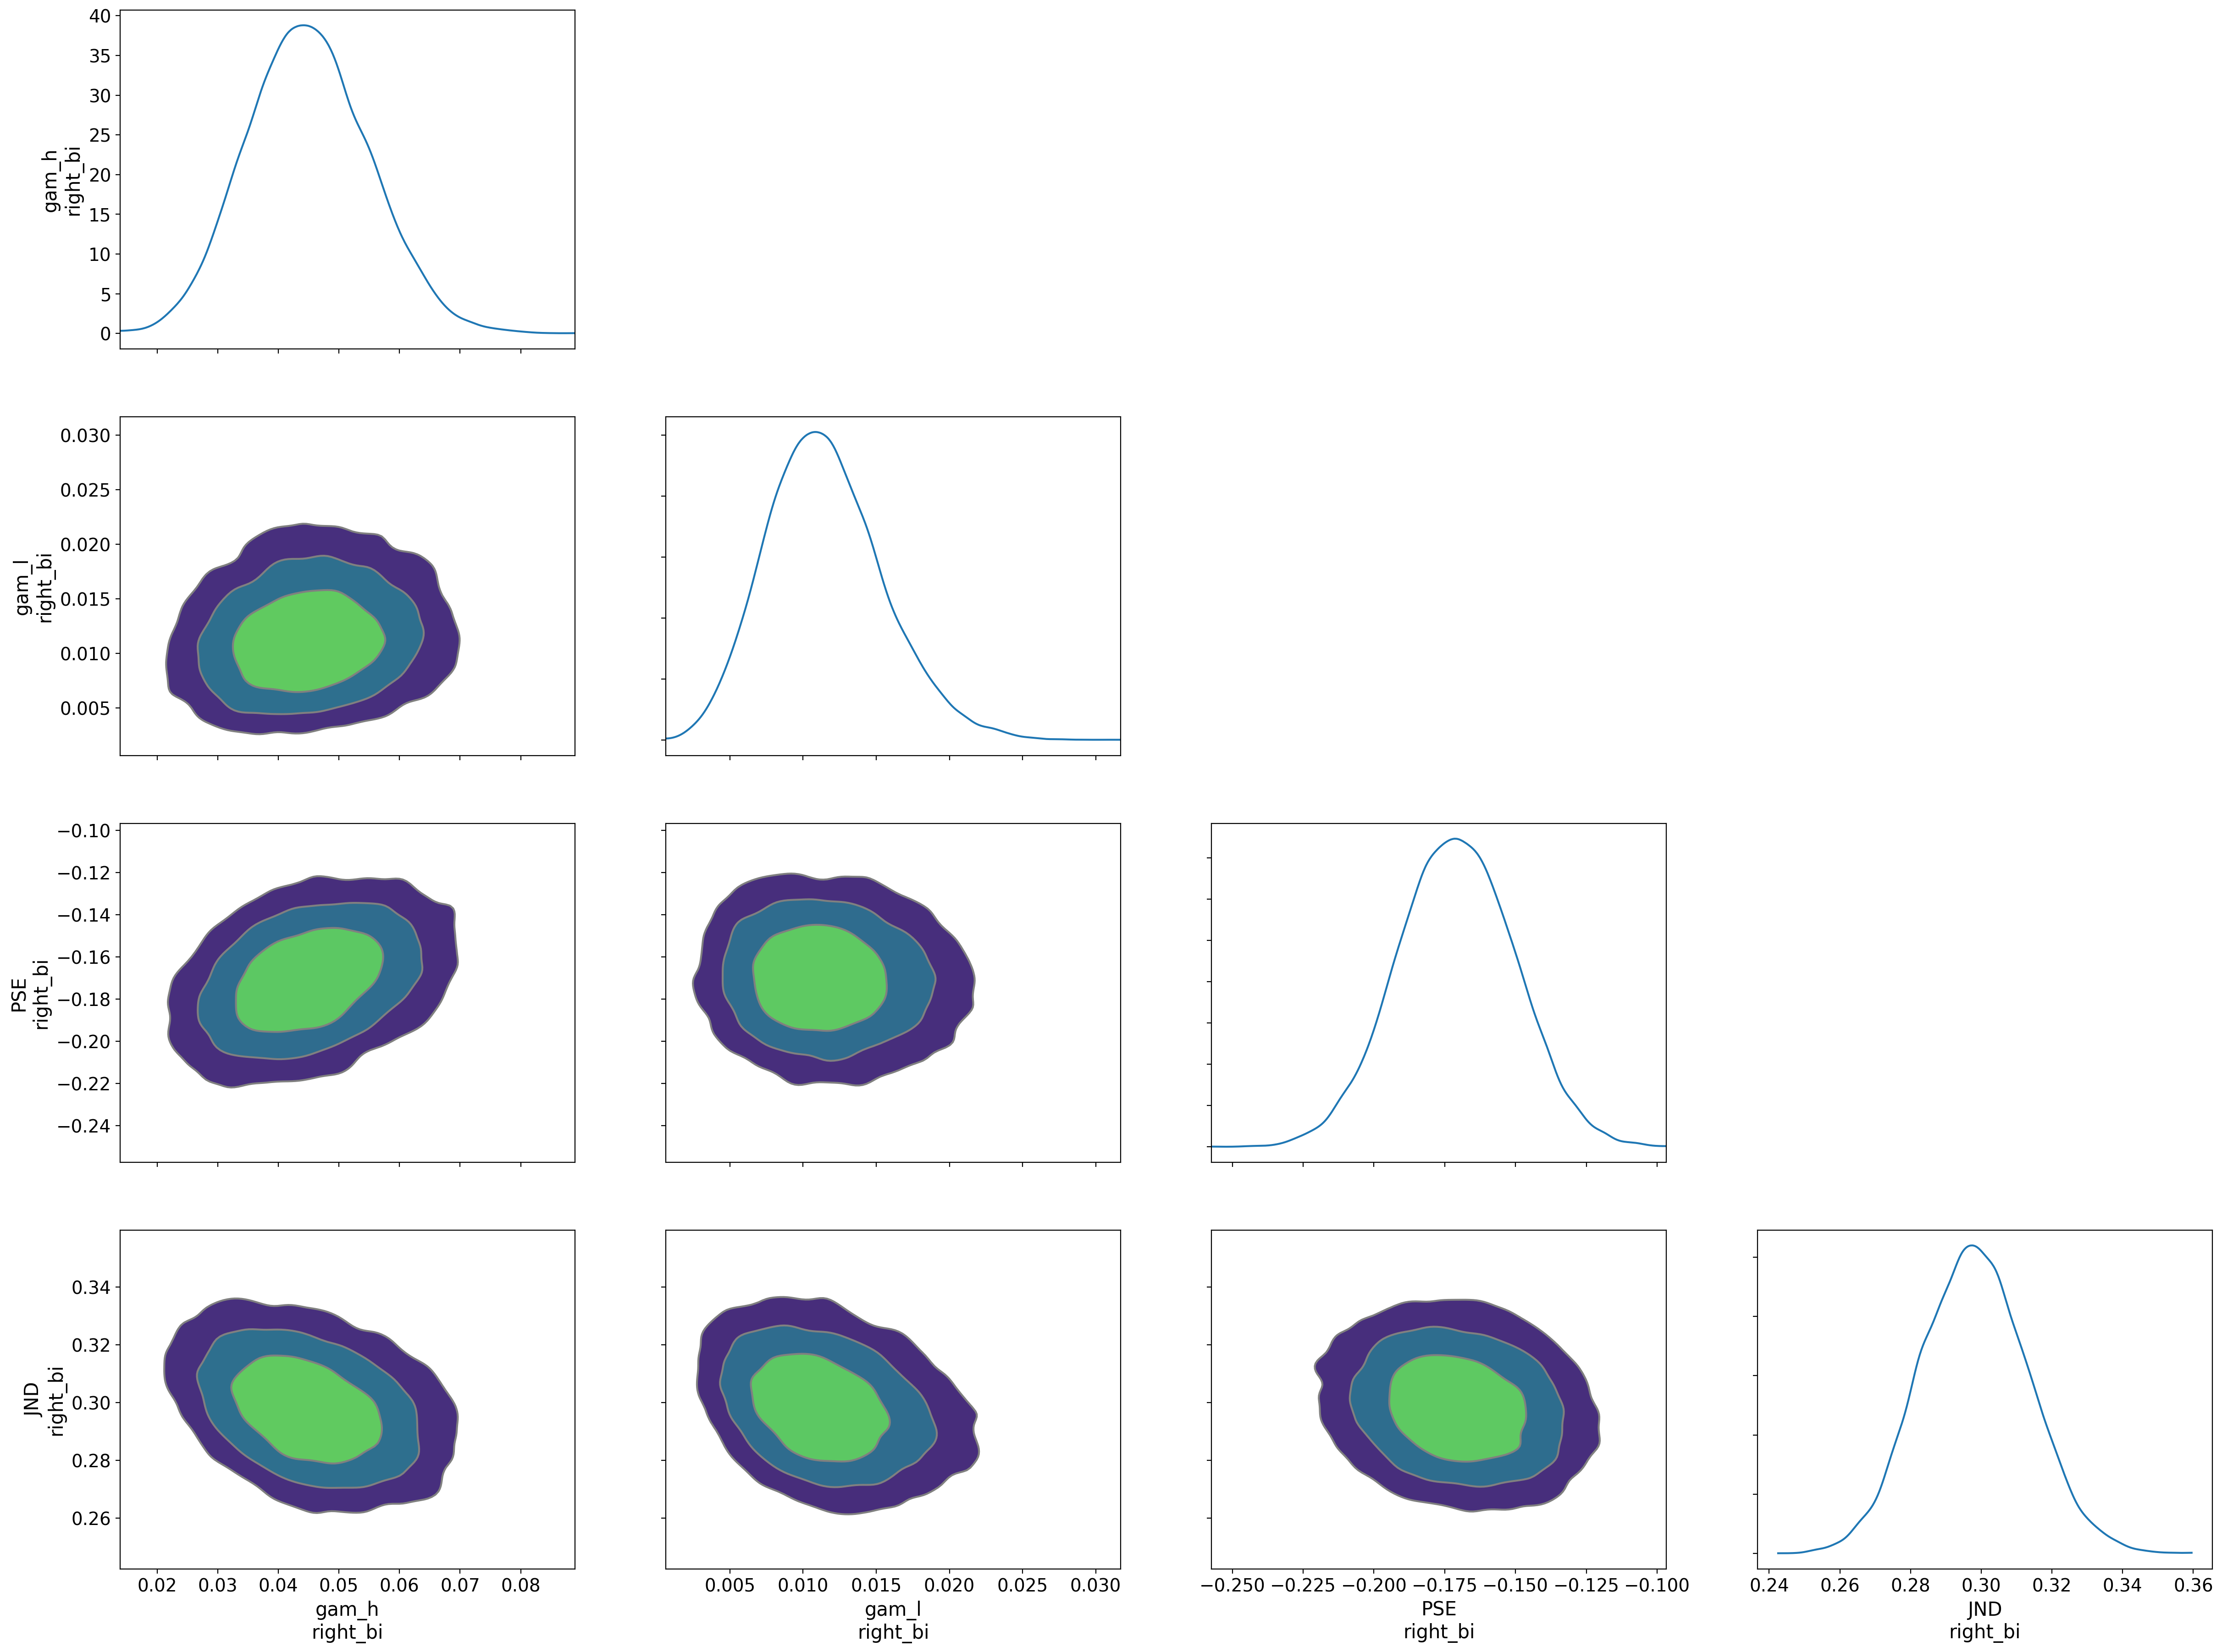
\includegraphics[width=0.48\textwidth]{pair_right_bi.png}
\caption{Joint posteriors of $\gamma_h$, $\gamma_l$, PSE and JND (standardized
units) for left\_uni, left\_bi (top) and right\_uni, right\_bi (bottom).}
\end{figure}

\end{document}
